% SIAM Article Template
\documentclass[review,onefignum,onetabnum]{siamart190516}

% Information that is shared between the article and the supplement
% (title and author information, macros, packages, etc.) goes into
% ex_shared.tex. If there is no supplement, this file can be included
% directly.

% SIAM Shared Information Template
% This is information that is shared between the main document and any
% supplement. If no supplement is required, then this information can
% be included directly in the main document.


% Packages and macros go here
\usepackage{lipsum}
\usepackage{amsfonts}
\usepackage{graphicx}
\usepackage{epstopdf}
\usepackage{amsmath}
\usepackage{subcaption}
\usepackage{pgfplots}

%\usepackage{amsmath,amsthm}
%\usepackage[noend]{algorithmic}
%\usepackage{algorithmic}
\usepackage[algo2e, ruled, noend, linesnumbered]{algorithm2e}
%\usepackage[algo2e, ruled, vlined]{algorithm2e}
\usepackage{bm}
\ifpdf
  \DeclareGraphicsExtensions{.eps,.pdf,.png,.jpg}
\else
  \DeclareGraphicsExtensions{.eps}
\fi

\usepackage{placeins}
\usepackage{multirow}

% Add a serial/Oxford comma by default.
\newcommand{\creflastconjunction}{, and~}
\newcommand{\nor}[1]{\left\|#1\right\|}

% Used for creating new theorem and remark environments
\newsiamremark{remark}{Remark}
\newsiamremark{hypothesis}{Hypothesis}
\crefname{hypothesis}{Hypothesis}{Hypotheses}
\newsiamthm{claim}{Claim}
\newsiamthm{prop}{Proposition}
\newsiamthm{defn}{Definition}
\newsiamthm{thm}{Theorem}
\newsiamthm{cor}{Corollary}
\newsiamthm{lem}{Lemma}


\newcommand{\norm}[1]{\|#1\|}


% Sets running headers as well as PDF title and authors
\headers{Matrix-free PSF approximation}{N. Alger, T. Hartland, N. Petra, and O. Ghattas}

% Title. If the supplement option is on, then "Supplementary Material"
% is automatically inserted before the title.
\title{Matrix-free point spread function approximation of operators with locally supported non-negative integral kernels, with application to Hessians in PDE constrained inverse problems\thanks{Submitted to the editors DATE.
\funding{This research was supported by the National Science Foundation under Grant No. DMS-1840265 and CAREER-1654311.}}}

% Authors: full names plus addresses.
\author{Nick Alger\thanks{Oden Institute, The University of Texas at Austin, Austin, TX 
  (\email{nalger@oden.utexas.edu}).}
\and Tucker Hartland\thanks{Department of Applied Mathematics, University of California, Merced, Merced, CA. 
	(\email{thartland@ucmerced.edu}).}
\and Noemi Petra\thanks{Department of Applied Mathematics, University of California, Merced, Merced, CA. 
  (\email{npetra@ucmerced.edu}).}
\and Omar Ghattas\thanks{Oden Institute, The University of Texas at Austin, Austin, TX 
	(\email{omar@oden.utexas.edu}).}}

\newcommand{\Aop}{\mathcal{A}}
\newcommand{\AopPc}{\mathcal{A}_\text{pc}}
\newcommand{\AopPcMesh}{\mathcal{A}_\text{pc}^h}

\newcommand{\Aker}{\Phi}
\newcommand{\AkerPc}{\Phi_\text{pc}}
\newcommand{\AkerPcMesh}{\Phi_\text{pc}^h}

\newcommand{\AkerPcMat}{\mathbf{\Phi}_\text{pc}}

\newcommand{\Amat}{\mathbf{A}}
\newcommand{\AmatPc}{\mathbf{A}_\text{pc}}
\newcommand{\AmatPcSym}{\mathbf{A}_\text{pc}^\text{sym}}
\newcommand{\AmatPcSymPlus}{\mathbf{A}_\text{pc}^{\text{sym}+}}

\newcommand{\diraccomb}{\xi}
\newcommand{\combresponse}{\eta}
\newcommand{\weakadmconst}{C}
\newcommand{\horizinterpolant}{\theta}
\newcommand{\interpolatedvalues}{b}
\newcommand{\firstgreens}{G}
\newcommand{\secondgreens}{F}
\newcommand{\impulseresponse}{\phi}
\newcommand{\convkernel}{\varphi}
\newcommand{\febasis}{\psi}
\newcommand{\ratfct}{R}
\newcommand{\ratpole}{\omega}
\newcommand{\ratcoeff}{c}
\newcommand{\massmatrix}{\mathbf{M}}
\newcommand{\spatialvol}{V}
\newcommand{\spatialmean}{\mu}
\newcommand{\spatialcov}{\Sigma}
\newcommand{\genericdistribution}{\rho}
\newcommand{\pointbatch}{S}
\newcommand{\pointinteractionmatrix}{S}
\newcommand{\gdim}{d}
\newcommand{\fedim}{N}
\newcommand{\convrank}{r}
\newcommand{\hrank}{k_h}
\newcommand{\nbatch}{n_b}
\newcommand{\numnbr}{k_{n}}
\newcommand{\ratord}{l}
\newcommand{\nsamplepts}{m}
\newcommand{\ptsonebatch}{s}
\newcommand{\classicalrank}{r}
\newcommand{\secondgreenscoeff}{\beta}
\newcommand{\constcoeff}{\alpha}
\newcommand{\colcluster}{\mathtt{c}}
\newcommand{\rowcluster}{\mathtt{r}}
\newcommand{\icedomain}{U}
\newcommand{\basalfriction}{{q}}
\newcommand{\normalvec}{\nu}
\newcommand{\searchdir}{{\widehat{\basalfriction}}}
\newcommand{\preconditioner}{\widetilde{H}}
\newcommand{\candidatepts}{X}
\newcommand{\eigenvectormatrix}{P}
\newcommand{\candidatepoint}{x}
\newcommand{\velocity}{v}
\newcommand{\pressure}{p}
\newcommand{\rbfweight}{c}
\newcommand{\stress}{\sigma}
\newcommand{\tangentop}{T}
\newcommand{\strain}{\varepsilon}
\newcommand{\bodyforce}{f}
\newcommand{\observations}{y}
\newcommand{\rbf}{\varphi}
\newcommand{\fepoint}{\zeta}
\newcommand{\stokesrobincoeff}{{s}}
\newcommand{\regrobincoeff}{{s}}
\newcommand{\regrhs}{{f}}

\newcommand*{\vertbar}{\rule[-1ex]{0.5pt}{2.5ex}}
\newcommand*{\horzbar}{\rule[.5ex]{2.5ex}{0.5pt}}

\usepackage{amsopn}
\DeclareMathOperator{\diag}{diag}
\DeclareMathOperator{\interpolate}{Interpolate}
\DeclareMathOperator{\Span}{span}
\DeclareMathOperator{\Var}{Var}
\DeclareMathOperator{\vol}{vol}
\DeclareMathOperator{\avg}{avg}
\DeclareMathOperator*{\argmax}{arg\,max}
\DeclareMathOperator*{\argmin}{arg\,min}
\DeclareMathOperator{\dist}{dist}
\DeclareMathOperator{\diam}{diam}
\DeclareMathOperator{\nbrs}{nbrs}

\newcommand{\computediracresponse}[1]{\text{compute\_dirac\_comb\_response}\left( #1 \right)}
\newcommand{\ellipsoidsintersect}[2]{\text{ellipsoids\_intersect}\left( #1, #2 \right)}
\newcommand{\choosebatch}[1]{\text{choose\_sample\_point\_batch}\left( #1 \right)}
\newcommand{\computekernelentries}[2]{\text{compute\_approximate\_kernel\_entries}\left( #1 , #2 \right)}
\newcommand{\computeweightingentries}[1]{\text{compute\_weighting\_function\_entries}\left( #1 \right)}

\DeclareFontFamily{U}{wncy}{}
\DeclareFontShape{U}{wncy}{m}{n}{<->wncyr10}{}
\DeclareSymbolFont{mcy}{U}{wncy}{m}{n}
\DeclareMathSymbol{\Sh}{\mathord}{mcy}{"58} 

\SetEndCharOfAlgoLine{}
%\SetKwIF{If}{ElseIf}{Else}{if}{}{else if}{else}{end if}

%\renewcommand{\algorithmicrequire}{\textbf{Input:}}
%\renewcommand{\algorithmicensure}{\textbf{Output:}}


%%% Local Variables: 
%%% mode:latex
%%% TeX-master: "ex_article"
%%% End: 


% Optional PDF information
\ifpdf
\hypersetup{
  pdftitle={Point spread function approximation of high rank Hessians with locally supported non-negative integral kernels},
  pdfauthor={N. Alger, N. Petra, T. Hartland, and O. Ghattas}
}
\fi

% The next statement enables references to information in the
% supplement. See the xr-hyperref package for details.

\externaldocument{localpsf_supplement}

% FundRef data to be entered by SIAM
%<funding-group specific-use="FundRef">
%<award-group>
%<funding-source>
%<named-content content-type="funder-name"> 
%</named-content> 
%<named-content content-type="funder-identifier"> 
%</named-content>
%</funding-source>
%<award-id> </award-id>
%</award-group>
%</funding-group>


\newcommand{\todo}[1]{\noindent\emph{\textcolor{red}{To do: #1\:}}}


\begin{document}

\maketitle

% REQUIRED
\begin{abstract}
	We present an efficient matrix-free point spread function (PSF) method for approximating operators that have locally supported non-negative integral kernels. The method computes impulse responses of the operator at a collection of scattered points, and interpolates translated and scaled versions of these impulse responses to approximate entries of the integral kernel. By applying the operator to Dirac combs associated with batches of point sources, we compute a large number of impulse responses using a small number of operator applications. We solve an ellipsoid packing problem to select as many point sources as possible per batch, while ensuring that the supports of the impulse responses within each batch do not overlap. Support ellipsoids are estimated a-priori based on impulse response moments, which are computed by applying the operator to a small number of polynomial functions. The interpolation uses a local mean displacement invariance approximation, which generalizes classical local translation invariance. The ability to rapidly evaluate kernel entries allows us to construct a hierarchical matrix (H-matrix) approximation of the operator. Further matrix computations such as matrix vector products, matrix-matrix additions, matrix factorizations, and the solution of linear systems are performed with H-matrix methods. 
	
	We demonstrate the effectiveness of the proposed method by using it to build preconditioners for the Hessian operator arising in two inverse problems governed by partial differential equations (PDEs): inversion for the basal friction coefficient in an ice sheet flow problem and inversion for the initial condition in a diffusive transport problem.
	While for many ill-posed inverse problems the Hessian of the data misfit term exhibits a low rank structure, and hence a low rank approximation is suitable, for many problems of practical interest the numerical rank of the Hessian is still large. This makes conventional matrix-free Hessian approximation methods expensive in terms of the required number of Hessian operator applications (hence PDE solves). In contrast, the performance of the proposed method depends on the locality and shapes of the impulse responses rather than the numerical rank. Hessian impulse responses typically become more local as the numerical rank increases, which makes high rank Hessians perfect candidates for the proposed approach. 
%	To demonstrate the effectiveness of the approximation, w
%	We use the proposed approach to build preconditioners to accelerate the solution of the inverse problems. 
%	We compare the results with classical regularization-based preconditioning and no preconditioning. 
%	The numerical results demonstrate the superior performance (measured in number of PDE solves) of the inverse solver when
	We observe that using the proposed PSF-based preconditioner clusters the spectrum of the preconditioned Hessian near one, yielding roughly 5X-10X reductions in the number of PDE solves required to solve the inverse problems, as compared to classical regularization-based preconditioning and no preconditioning. Finally, we present a comprehensive numerical study for the influence of the diffusion parameters and simulation time (for the diffusive transport problem) on the effectiveness of the approximation. These parameters have an effect on the shape of the impulse responses and on the rank of the Hessian. The results reveal that PSF-based preconditioners are able to form good approximations of high-rank Hessians using a small number of operator applications.
\end{abstract}

% REQUIRED
\begin{keywords}
 	data scalability, Hessian, hierarchical matrix, matrix-free, operator approximation, PDE constrained inverse problems, point spread function, product convolution, local translation invariance, impulse response, moment methods, high-rank
\end{keywords}

% REQUIRED
\begin{AMS}
 	35R30, 41A35, 47A52, 47J06, 65D12, 65F08, 65F10, 65K10, 65N21, 86A22, 86A40
\end{AMS}

\section{Introduction}
\label{sec:intro}

We present an efficient \emph{matrix-free} point spread function (PSF) method for approximating operators $\Aop:L^2(\Omega) \rightarrow L^2(\Omega)'$ that have locally supported non-negative integral kernels. Here $\Omega \subset \mathbb{R}^\gdim$ is a bounded domain, and $L^2(\Omega)'$ is the space of real-valued continuous linear functionals on $L^2(\Omega)$. Such operators appear, for instance, as Hessians in optimization and inverse problems governed by partial differential equations (PDEs)~\cite{AntilEtAl18,BorziSchulz11,Delosreyes15,HinzePinnauUlbrichUlbrich08}, Schur complements in Schur complement methods for solving partial differential equations (PDEs) and Poincare-Steklov operators in domain decomposition methods (e.g., Dirichlet-to-Neumann maps)~\cite{ChanMathew94,SmithBjorstadGropp96,ToselliWidlund04}, covariance operators in spatial statistics~\cite{ChenStein21,GentonKeyesTurkiyyah18,GeogaEtAl20,LindgrenRueLindstrom11}, and blurring operators in imaging~\cite{DenisEtAl11,NagyOleary98}. Here ``matrix-free'' means that we may apply $\Aop$ and its transpose\footnote{Recall that $\Aop^T:L^2(\Omega)\rightarrow L^2(\Omega)'$ is the unique operator satisfying $\left(\Aop u\right)(w) = \left(\Aop^T w\right)(u)$ for all $u,w \in L^2(\Omega)$, where $\Aop u \in L^2(\Omega)'$ is the result of applying $\Aop$ to $u\in L^2(\Omega)$, and $\left(\Aop u\right)(w)$ is the result of applying that linear functional to $w \in L^2(\Omega)$, and similar for operations with $\Aop^T$. }, $\Aop^T$, to functions,
\begin{equation}
\label{eq:eval_maps}
u \mapsto\Aop u \qquad \text{and} \qquad w \mapsto \Aop^T w,
\end{equation} 
via a black box computational procedure, 
but cannot easily access entries of $\Aop$'s integral kernel. Evaluating the maps in~\eqref{eq:eval_maps} may require solving a subproblem that involves PDEs, or performing other costly computations. By ``non-negative integral kernel,'' we mean that entries of the integral kernel are non-negative numbers; this is not the same as positive semi-definiteness of $\Aop$.




\begin{figure}
	\begin{subfigure}{0.32\textwidth}
		\centering
		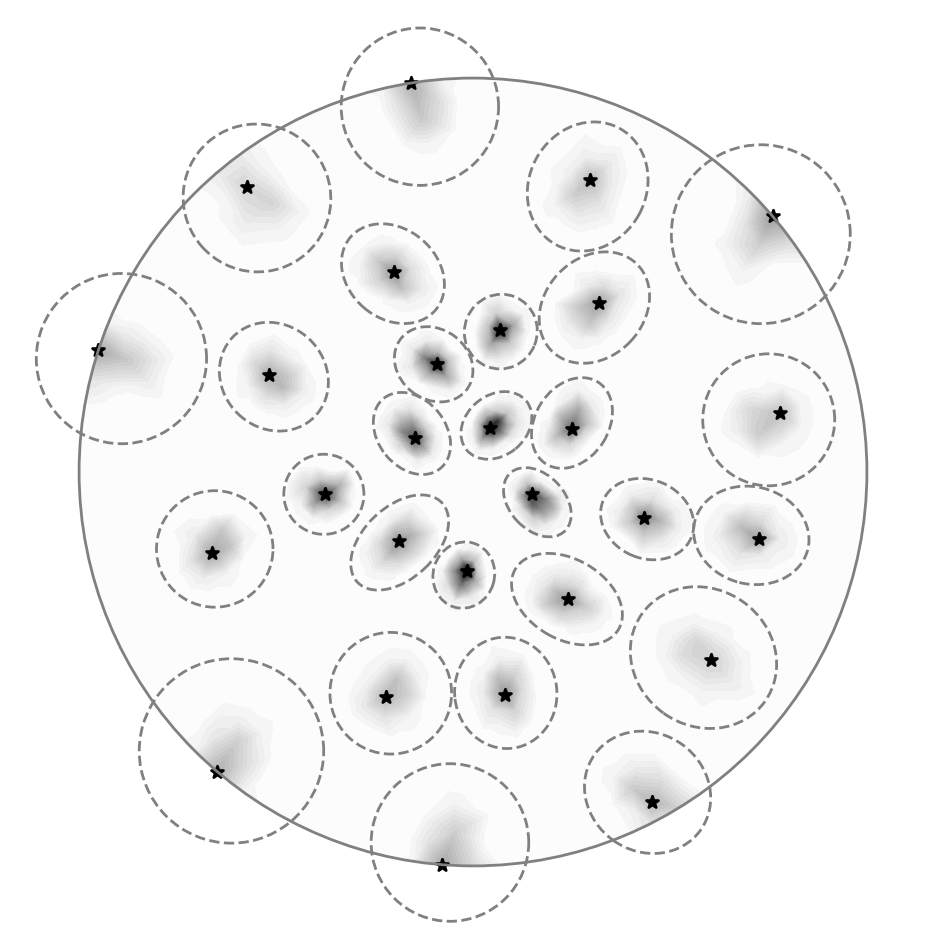
\includegraphics[scale=0.34]{impulse_batch1.png}
	\end{subfigure}
	\begin{subfigure}{0.32\textwidth}
		\centering
		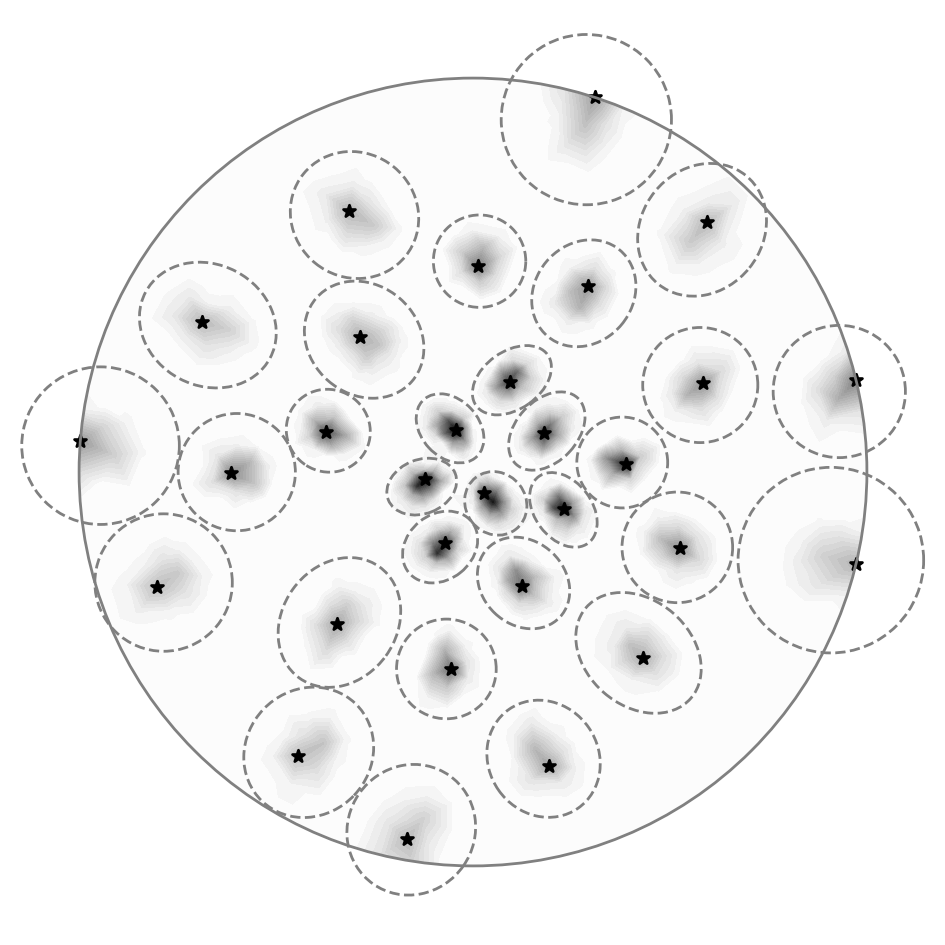
\includegraphics[scale=0.34]{impulse_batch2.png}
	\end{subfigure}
	\begin{subfigure}{0.32\textwidth}
		\centering
		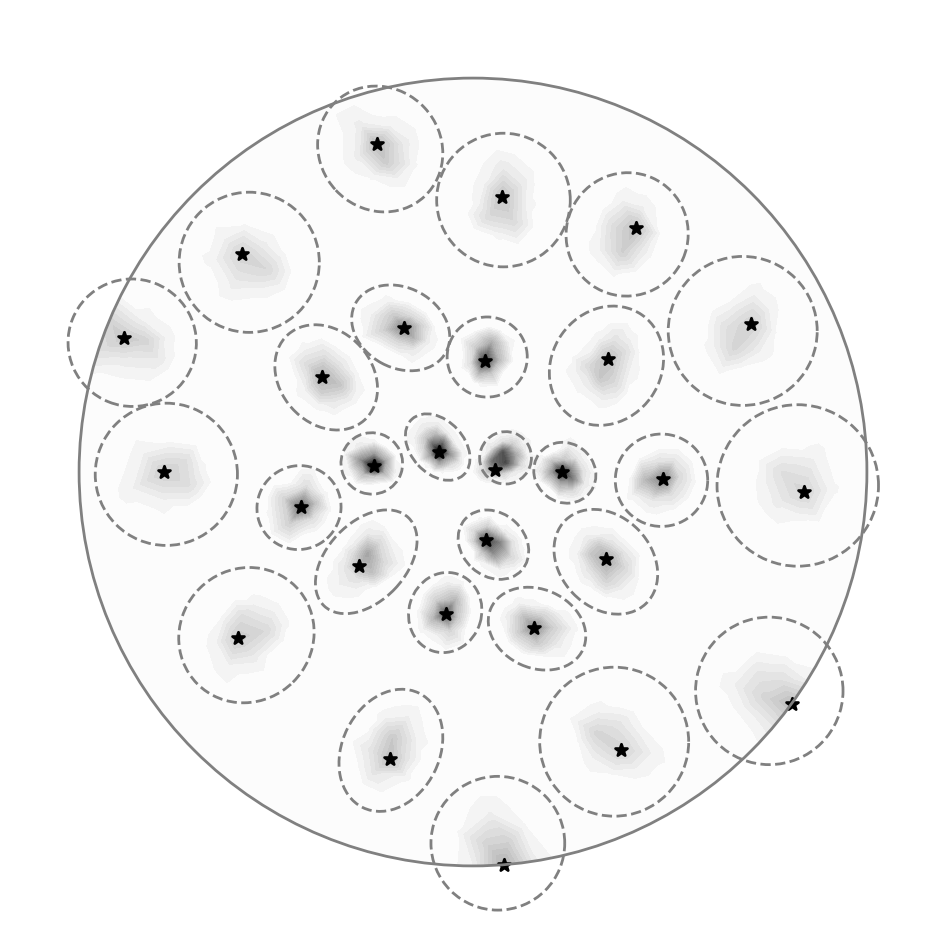
\includegraphics[scale=0.34]{impulse_batch3.png}
	\end{subfigure}
	\caption{Three batches, $\eta_b$, of normalized impulse responses, $\impulseresponse_{x}$, that arise from applying $\Aop$ to weighted sums of scattered point sources (see Section \ref{sec:get_impulse_response}). Here $\Aop$ is the ice sheet inverse problem data misfit Gauss-Newton Hessian described in Section~\ref{sec:numerical_results}. 
	Black stars are point source locations. Shading shows the magnitude of the normalized impulse responses (darker means larger function values). Dashed gray ellipses are estimated impulse response support ellipsoids based on the moment method in Section \ref{sec:intromoments}. The large circle is $\partial \Omega$. 
	}
	\label{fig:batches_intro}
\end{figure}

We use \emph{impulse response interpolation} to form a high rank approximation of $\Aop$ using a small number of operator applications. The impulse response, $\phi_x$, associated with a point, $x$, is the Riesz representation\footnote{Recall that the Riesz representative of a functional $\rho \in L^2(\Omega)'$ with respect to the $L^2$ inner product is the unique function $\rho^* \in L^2(\Omega)$ such that $\rho(w) = \left(\rho^*,w\right)_{L^2(\Omega)}$ for all $w \in L^2(\Omega)$.} of the linear functional that results from applying $\Aop$ to a delta distribution (i.e., point source, impulse) centered at $x$. We compute batches of impulse responses by applying $\Aop$ to weighted sums of delta distributions associated with batches of points scattered throughout the domain (see Figure~\ref{fig:batches_intro}). Then we interpolate translated and scaled versions of these impulse responses to approximate entries of the operator's integral kernel. 
Picking the batches of points requires us to estimate the supports of the impulse responses $\phi_x$ \emph{before} they are computed. Ellipsoid estimates for the supports of all $\phi_x$ are determined a-priori via a moment method that involves applying $\Aop^T$ to a small number of polynomial functions (see Section~\ref{sec:intromoments}). We are inspired by resolution analysis in seismic imaging, in which
$\Aop^T$ is applied to a random noise function, and the width of the support $\phi_x$ is estimated to be the autocorrelation length of the resultant function near $x$~\cite{FichtnerLeeuwen15,TrampertFichtnerRitsema13}. The moment method that we use estimates the support of $\phi_x$ more accurately than random noise probing in resolution analysis, at the cost of the additional constraint that $\Aop$ has a non-negative integral kernel. 

The proposed operator approximation method may be categorized as a PSF method that is loosely based on ``product convolution'' (PC) approximations, which are approximations of an operator by weighted sums of convolution operators with spatially varying weights. PC and PSF methods have a long history dating back several decades. We note the following papers (among many others) in which the convolution kernels are constructed from sampling impulse responses of the operator to scattered point sources:~\cite{Adorf94,AlgerEtAl19,BigotEscandeWeiss19,EscandeWeiss15,EscandeWeiss22,EscandeWeiss12,FishEtAl96,NagyOleary98,ZhuLiFomelEtAl16}. For background on PC and PSF methods, we recommend the following papers: \cite{DenisEtAl15,EscandeWeiss17,GentileCourbinMeylan13}. While PC approximations are based on an assumption of local translation invariance, the method we propose is based on a more general assumption we call ``local mean displacement invariance'' (Section~\ref{sec:local_mean_displacement_invariance} and Figure~\ref{fig:mean_displacement_invariance}). This improves the interpolation of the impulse responses. Furthermore, in our previous work~\cite{AlgerEtAl19}, we chose point sources optimally via a sequential adaptive procedure. However, in that work each point source required a separate operator application, making the previous method expensive when a large number of impulse responses is desired. In this paper, we use a new moment method (Section \ref{sec:intromoments}) which permits computation of many impulse responses (e.g., 50) per operator application. Finally, the method we propose never evaluates computed impulse responses outside of their domain of definition. This eliminates boundary artifacts which plague conventional PC methods.


\begin{figure}
	\begin{center}
		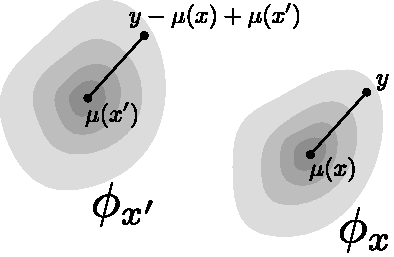
\includegraphics[scale=0.75]{mean_displacement_invariance.pdf}
	\end{center}
	\caption{This figure illustrates impulse responses, $\impulseresponse_x$ and $\impulseresponse_{x'}$, that arise from applying $\Aop$ to point sources at two points, $x$ and $x'$. The operator $\Aop$ is locally mean displacement invariant (Section \ref{sec:local_mean_displacement_invariance}) if $\impulseresponse_{x}(y) \approx \impulseresponse_{x'}\left(y - \spatialmean(x) + \spatialmean(x')\right)$ when $x$ is close to $x'$. Here $\spatialmean(z)$ denotes the mean (center of mass) of $\phi_z$.}
	\label{fig:mean_displacement_invariance}
\end{figure}

The ability to rapidly approximate entries of $\Aop$'s integral kernel allows one to approximate discretized versions of $\Aop$ using the full arsenal of tools for matrix approximation that rely on fast access to matrix entries.
In this work, we form a hierarchical matrix (H-matrix)~\cite{BormGrasedyckHackbusch03,Hackbusch99} approximation of a discretized version of $\Aop$. H-matrices are a matrix format in which the rows and columns of the matrix are re-ordered, then the matrix is recursively subdivided into blocks in such a way that many off-diagonal blocks are low rank, even though the matrix as a whole may be high rank. 
H-matrix methods permit us to perform matrix-vector products cheaply, and perform other useful linear algebra operations that cannot be done easily using the original operator. These operations include matrix-matrix addition, matrix-matrix multiplication, matrix factorization, and matrix inversion. 
The work and memory required to perform these operations for an $\fedim \times \fedim$ H-matrix scales 
\emph{nearly linearly} in $N$ (i.e., $o(N^{1+\epsilon})$ for any $\epsilon > 0$). The exact cost depends on the type of H-matrix used, the operation being performed, and the rank of the off-diagonal blocks~\cite{GrasedyckHackbusch03}. 


\section{Why we need more efficient approximations of high rank Hessians}
\label{sec:hessian}

In distributed parameter inverse problems governed by PDEs, one seeks to infer an unknown spatially varying parameter field from limited observations of a state variable that depends on the parameter implicitly through the solution of a PDE. 
Conventionally, the inverse problem is formulated using either a deterministic framework~\cite{AsterBorchersThurber18,BanksKunisch89,Vogel02},
or a Bayesian probabilistic framework~\cite{KaipioSomersalo05,Stuart10a,Tarantola05}. In the deterministic framework, one solves an optimization problem to find the parameter that best fits the observations, subject to appropriate regularization~\cite{EnglHankeNeubauer96,Vogel02}. In the probabilistic framework, Bayes' theorem combines the observations with prior information to form a posterior distribution over the space of all possible parameter fields, and computations are performed to extract statistical information about the parameter from this posterior. The Hessian of the objective function with respect to the parameter in the determinstic optimization problem and the Hessian of the negative log posterior in the Bayesian setting are equal or approximately equal under typical noise, regularization, and prior models, so we refer to both of these Hessians as ``the Hessian.'' The Hessian consists of a data misfit term (the \emph{data misfit Hessian}), which depends on a discrepancy between the observations and the associated model predictions, and a regularization or prior term (the \emph{regularization Hessian}) which does not depend on the observations. For more details on the Hessian, see~\cite{Alger19,GhattasWillcox21,VillaPetraGhattas21}. 

Hessian approximations and preconditioners are highly desirable because the Hessian is central to efficient solution of inverse problems in both the deterministic and Bayesian settings. When solving the deterministic optimization problem with Newton-type methods, the Hessian is the coefficient operator for the linear system that must be solved or approximately solved at every Newton iteration. Good Hessian preconditioners reduce the number of iterations required to solve these Newton linear systems with the conjugate gradient method~\cite{Saad03}. In the Bayesian setting, the inverse of the Hessian is the covariance of a local Gaussian approximation of the posterior. This Gaussian distribution can be used directly as an approximation of the posterior, or it can be used as a proposal for Markov chain Monte-Carlo methods for drawing samples from the posterior. For instance, see~\cite{KimEtAl21,PetraEtAl14} and the references therein. 

Owing to the implicit dependence of predicted observations on the parameter, entries of the Hessian are not easily accessible. Rather, the Hessian may be applied to a vector via a computational process that involves solving a pair of forward and adjoint PDEs which are linearizations of the original PDE~\cite{GhattasWillcox21}
%,Gunzburger03}
. The most popular matrix-free Hessian approximation methods are based on low rank approximation of either the data misfit Hessian, or the data misfit Hessian preconditioned by the regularization Hessian, e.g.,~\cite{BuiEtAl13,CuiEtAl14,FlathEtAl11,PetraEtAl14,SpantiniEtAl15}. Krylov methods such as Lanczos or randomized methods~\cite{Cheng05,HalkoMartinssonTropp11} are typically used to construct these low rank approximations by applying the Hessian to vectors. Using these methods, the required number of Hessian applications (and hence the required number of PDE solves) is proportional to the rank of the low rank approximation. Low rank approximation methods are justified by arguing that the numerical rank of the data misfit Hessian is insensitive to the dimension of the discretized parameter. This means that the required number of PDE solves remains the same as the mesh used to discretize the parameter is refined.
However, in many inverse problems of practical interest the numerical rank of the data misfit Hessian, while mesh independent, is still large, which makes it costly to approximate the Hessian using low rank approximation methods~\cite{AmbartsumyanEtAl20,BuiEtAl13,IsaacEtAl15}. 

Examples of inverse problems with high rank data misfit Hessians include large-scale ice sheet inverse problems \cite{HartlandEtAl23,IsaacEtAl15}, advection dominated advection-diffusion inverse problems~\cite{AkcelikBirosDraganescuEtAl05}\cite[Chapter 5]{Flath13}, high frequency wave propagation inverse problems~\cite{BuiEtAl13}, inverse problems governed by high Reynolds number flows, and more generally, all inverse problems in which the observations highly inform the parameter. The eigenvalues of the data misfit Hessian characterize how informative the data are about components of the parameter in the corresponding eigenvector directions,
hence more informative data leads to larger eigenvalues and a larger numerical rank~\cite{AlexanderianGloorGhattas16}\cite[Section 1.4 and Chapter 4]{Alger19}. Roughly speaking, the numerical rank of the data misfit Hessian is the dimension of the subspace of parameter space that is informed by the data. The numerical rank of the regularization preconditioned data misfit Hessian may be reduced by increasing the strength of the regularization, but this throws away useful information: components of the parameter that could be learned from the observations
would instead be reconstructed based on the regularization~\cite[Section 4]{AlgerEtAl17}\cite[Chapters 1 and 7]{Vogel02}. Hence, low rank approximation methods suffer from a predicament: if the data highly inform the parameter and the regularization is chosen appropriately, then a large number of operator applications are required to form an accurate approximation of the Hessian using low rank approximation methods. 
High rank Hessian approximation methods are thus needed.

Recently there have been improvements in matrix-free H-matrix construction methods in which an operator is applied to structured random vectors, and the response of the operator to those random vectors is processed to construct an H-matrix approximation~\cite{LevittMartinsson22,LinYing11,Martinsson11,Martinsson16,MartinssonTropp20}. 
These methods (which we do not use here) have been used to approximate Hessians in PDE constrained inverse problems~\cite{AmbartsumyanEtAl20,HartlandEtAl23}. 
Although these methods are promising,
the required number of operator applications is still large (e.g., hundreds to thousands).
In this paper, we also form an H-matrix Hessian approximation. However, to reduce the required number of operator applications, we first form a PSF approximation of the data misfit Hessian by exploiting locality and non-negative integral kernel properties, then form the H-matrix using classical H-matrix techniques. By using this two stage approach, we reduce the number of operator applications to a few dozen at most. One limitation of our method is that not all data misfit Hessians satisfy the local non-negative integral kernel properties (for example, the wave inverse problem data misfit Hessian has a substantial amount of negative entries in its integral kernel). However, many data misfit Hessians of practical interest do satisfy these properties (either exactly or approximately), and the proposed method is targeted at approximating these Hessians.


\section{Preliminaries}

Let $\Omega \subset \mathbb{R}^\gdim$ be a bounded domain (typically $\gdim=1$, $2$, or $3$). We seek to approximate integral operators $\Aop:L^2(\Omega)\rightarrow L^2(\Omega)'$ of the form
\begin{equation}
\label{eq:kernel_representation}
(\Aop u)(w) := \int_\Omega \int_\Omega w(y) \Aker(y,x) u(x) \mathrm{d}x \mathrm{d}y.
\end{equation}
The linear functional $\Aop u \in L^2(\Omega)'$ is the result of applying $\Aop$ to $u\in L^2(\Omega)$, and the scalar $\left(\Aop u\right)(w)$ is the result of applying that linear functional to $w \in L^2(\Omega)$.
The integral kernel, $\Aker:\Omega \times \Omega \rightarrow \mathbb{R}$, exists but is not easily accessible. In this section we describe how to extend the domain of $\Aop$ to distributions, which allows us to define impulse responses (Section~\ref{sec:impulse_response_2}), we then state the conditions on $\Aop$ that the proposed method requires (Section~\ref{sec:conditions_2}), and detail finite element discretization (Section~\ref{sec:finite_element_kernel}).

\subsection{Distributions and impulse responses}
\label{sec:impulse_response_2}

The operator $\Aop$ may be applied to distributions if $\Aker$ is sufficiently regular. 
Given $\rho \in L^2(\Omega)'$, let $\rho^* \in L^2(\Omega)$ denote the Riesz representative of $\rho$ with respect to the $L^2(\Omega)$ inner product. We have
\begin{subequations}
	\label{eq:extension_to_distributions}
	\begin{align}
		\left(\Aop \genericdistribution^*\right)(w) &= \int_\Omega \int_\Omega w(y) \Aker(y,x) \genericdistribution^*(x) \mathrm{d}x ~\mathrm{d}y \\
		&= \int_\Omega w(y) \int_\Omega \Aker(y,x) \genericdistribution^*(x) \mathrm{d}x ~\mathrm{d}y 
		= \int_\Omega w(y) \genericdistribution\left(\Aker(y,\cdot)\right) \mathrm{d}y, \label{eq:action_on_distribution}
	\end{align}
\end{subequations}
where $\Aker(y,\cdot)$ denotes the function $x \mapsto \Aker(y,x)$.
Now let $\mathcal{D}(\Omega) \subset L^2(\Omega)$ be a suitable space of test functions and let $\rho:\mathcal{D}(\Omega) \rightarrow \mathbb{R}$ be a distribution. In this case, 
$\rho^*$ may not exist, so the derivation in~\eqref{eq:extension_to_distributions} is not valid. However, if $\Aker$ is sufficiently regular such that the function $y \mapsto \rho\left(\Aker(y,~\cdot~)\right)$ is well-defined for almost all $y\in\Omega$, and if this function is in $L^2(\Omega)$, then the right hand side of~\eqref{eq:action_on_distribution} is well-defined. Hence, we \emph{define} the application of $\Aop$ to the distribution $\rho$ to be the right hand side of~\eqref{eq:action_on_distribution}. We denote this operator application by ``$\Aop \genericdistribution^*$,'' even if $\rho^*$ does not exist.

Let $\delta_x$ denote the delta distribution\footnote{Recall that the delta distribution $\delta_x:\mathcal{D}(\Omega)\rightarrow \mathbb{R}$ is defined by $\delta_x(w) = w(x)$ for all $w\in \mathcal{D}(\Omega)$.} (i.e., point source, impulse) centered at the point $x \in \Omega$.
The \emph{impulse response} of $\Aop$ associated with $x$ is the function $\impulseresponse_x:\Omega \rightarrow \mathbb{R}$, 
\begin{equation}
\label{eq:impulse_response_delta_action}
\impulseresponse_x := \left( \Aop \delta_x^* \right)^*,
\end{equation}
that is formed by applying $\Aop$ to $\delta_x$, then taking the Riesz representation of the resulting linear functional. Using~\eqref{eq:action_on_distribution} and the definition of the delta distribution, we see that $\phi_x$ may also be written as the function $\impulseresponse_x(y) = \Aker(y, x)$.

\subsection{Required conditions}
\label{sec:conditions_2}

We focus on approximating operators that satisfy the following conditions: 
\begin{enumerate}
	\item The kernel $\Aker$ is sufficiently regular so that $\phi_x$ is well-defined for all $x\in \Omega$.
	\item The supports of the impulse responses $\impulseresponse_x$ are contained in localized regions.
	\item The integral kernel is non-negative in the sense that $$\Aker(y,x) \ge 0$$ for all $(y,x) \in \Omega \times \Omega$.\footnote{Note that having a non-negative integral kernel is different from positive semi-definiteness. The operator $\Aop$ need not be positive semi-definite to use the proposed method, and positive semi-definite operators need not have a non-negative integral kernel.}
\end{enumerate}
The proposed method may still perform well if these conditions are relaxed slightly. It is acceptable if the support of $\impulseresponse_x$ is not perfectly contained in a localized region, so long as the bulk of the ``mass'' of $\impulseresponse_x$ is contained in a localized region. The integral kernel does not need to be non-negative for all pairs of points $(y,x) \in \Omega \times \Omega$ so long as it is non-negative for the vast majority of pairs of points $(y,x)$, and so long as the negative numbers are comparatively small. If these conditions are violated, the method will incur additional error, and depending on the severity of the violation, the proposed method may fail.

\subsection{Finite element discretization}
\label{sec:finite_element_kernel}

In computations, functions are discretized and replaced by finite-dimensional vectors, and operators mapping between infinite-dimensional spaces are replaced by operators mapping between finite-dimensional spaces. In this paper we discretize using continuous Galerkin finite elements satisfying the Kronecker property (defined below). With minor modifications, the proposed method could be used with more general finite element methods, or other discretization schemes such as finite differences or finite volumes.

Let $\febasis_1, \febasis_2, \dots, \febasis_\fedim$ be a set of continuous Galerkin finite element basis functions used to discretize the problem on a mesh with mesh size parameter $h$, let $V_h := \Span\left(\febasis_1, \febasis_2, \dots, \febasis_\fedim\right)$ be the corresponding finite element space under the $L^2$ inner product, and let $\fepoint_i \in \mathbb{R}^\gdim$, $i=1,\dots, \fedim$ be the Lagrange nodes associated with the functions $\febasis_i$. We assume that the finite element basis satisfies the Kronecker property, i.e., $\febasis_i(\fepoint_i)=1$ and $\febasis_i(\fepoint_j)=0$ if $i\neq j$. 
For $u_h \in V_h$ we write $\bm{u} \in \mathbb{R}^\nsamplepts_\massmatrix$ to denote the coefficient vector for $u_h$ with respect to the finite element basis, i.e.,
$
u_h(x) = \sum_{i=1}^\fedim \bm{u}_i \febasis_i(x).
$
Linear functionals $\rho_h \in V_h'$ have coefficient dual vectors $\boldsymbol{\rho}\in \mathbb{R}^\nsamplepts_{\massmatrix^{-1}}$, with entries $\boldsymbol{\rho}_i = \rho_h(\febasis_i)$ for $i=1,\dots,\nsamplepts$.
Here $\massmatrix \in \mathbb{R}^{\fedim \times \fedim}$ denotes the sparse finite element mass matrix which has entries $\massmatrix_{ij}=\int_\Omega \febasis_i(x) \febasis_j(x) \mathrm{d}x$ for $i,j=1,\dots,\fedim$.
The space $\mathbb{R}^\fedim_\massmatrix$ is $\mathbb{R}^\fedim$ with the inner product $(\mathbf{u},\mathbf{w})_\massmatrix := \mathbf{u}^T \massmatrix \mathbf{w}$, and $\mathbb{R}^\fedim_{\massmatrix^{-1}}$ is the analogous space with $\massmatrix^{-1}$ replacing $\massmatrix$. Direct calculation shows that $\mathbb{R}^\fedim_\massmatrix$ and $\mathbb{R}^\fedim_{\massmatrix^{-1}}$ are isomorphic to $V_h$ and $V_h'$ as Hilbert spaces, respectively.

After discretization, the operator $\Aop:L^2(\Omega) \rightarrow L^2(\Omega)'$ is replaced by an operator $A_h:V_h \rightarrow V_h'$, which becomes an operator
$
\mathbf{A}:\mathbb{R}^\fedim_\massmatrix \rightarrow \mathbb{R}^\fedim_{\massmatrix^{-1}}
$
under the isomorphism discussed above. The proposed method is agnostic to the computational procedure for approximating $\Aop$ with $\mathbf{A}$. What is important is that we do not have direct access to matrix entries $\mathbf{A}_{ij}$. Rather, we have a computational procedure that allows us to compute matrix-vector products $\mathbf{u}\mapsto \mathbf{A}\mathbf{u}$ and $\mathbf{w}\mapsto \mathbf{A}^T\mathbf{w}$, and computing these matrix-vector products is costly. The proposed method mitigates this cost by performing as few matrix-vector products as possible.
Of course, matrix entries can be computed via matrix-vector products as $\mathbf{A}_{ij} = \left(\mathbf{A}\mathbf{e}_j\right)_i$,
where $\mathbf{e}_j=(0,\dots,0,1,0,\dots,0)^T$ is the length $\fedim$ unit vector with one in the $j$th coordinate and zeros elsewhere. But computing the matrix-vector product $\mathbf{e}_j \mapsto \mathbf{A}\mathbf{e}_j$ is costly, and therefore wasteful if we do not use other matrix entries in the $j$th column of $\mathbf{A}$. Hence, methods for approximating $\mathbf{A}$ are computationally intractable if they require accessing scattered matrix entries from many different rows and columns of $\mathbf{A}$. 

The operator $A_h:V_h \rightarrow V_h'$ can be written in integral kernel form,~\eqref{eq:kernel_representation}, but with $\Aker$ replaced by a slightly different integral kernel,
$\Aker_h$, which we do not know, and which differs from $\Aker$ due to discretization error. Since the functions in $V_h$ are continuous at $x$, the delta distribution $\delta_x$ is a continuous linear functional on $V_h$, which has a discrete dual vector $\boldsymbol{\delta}_x \in \mathbb{R}^\fedim_{\massmatrix^{-1}}$ with entries $\left(\boldsymbol{\delta}_x\right)_i = \febasis_i(x)$ for $i=1,\dots,\fedim$. Additionally, it is straightforward to verify that the Riesz representation, $\rho_h^* \in V_h$, of a functional $\rho \in V_h'$ has coefficient vector
$
\boldsymbol{\rho}^* = \massmatrix^{-1} \boldsymbol{\rho}.
$
Therefore, the formula for the impulse response from~\eqref{eq:impulse_response_delta_action} becomes 
$
\boldsymbol{\impulseresponse}_x = \left(A_h \delta_x^*\right)^* =  \massmatrix^{-1}\mathbf{A} \massmatrix^{-1} \boldsymbol{\delta}_x,
$
and the $(y,x)$ kernel entry of $\Aker_h$ may be written as
$
	\Aker_h(y,x) = \boldsymbol{\delta}_y^T \boldsymbol{\impulseresponse}_x = \boldsymbol{\delta}_y^T \massmatrix^{-1}\mathbf{A} \massmatrix^{-1} \boldsymbol{\delta}_x.
$
Now define $\mathbf{\Aker} \in \mathbb{R}^{\fedim \times \fedim}$ to be the following dense matrix of kernel entries evaluated at all pairs of Lagrange nodes:
\begin{equation}
\label{eq:Akerpcmat_entries}
\mathbf{\Aker}_{ij} := \Aker_h(\fepoint_i, \fepoint_j).
\end{equation}
Because of the Kronecker property of the finite element basis, we have $\boldsymbol{\delta}_{\fepoint_i} = \mathbf{e}_i$. Thus, we have
$
	\Aker_h(\fepoint_i,\fepoint_j) = \left(\massmatrix^{-1}\mathbf{A} \massmatrix^{-1}\right)_{ij},
$
which implies
\begin{equation}
\label{eq:boldA}
	\mathbf{A} = \massmatrix \mathbf{\Aker} \massmatrix.
\end{equation}
Broadly, we will construct an H-matrix approximation of $\mathbf{A}$ by forming a H-matrix approximation of $\boldsymbol{\Aker}$, then multiplying $\boldsymbol{\Aker}$ by $\massmatrix$ (or a lumped mass version of $\massmatrix$) on the left and right using H-matrix methods. Classical H-matrix construction methods require access to arbitrary matrix entries $\mathbf{\Aker}_{ij}$, but these matrix entries are not easily accessible. The bulk of the proposed method is therefore dedicated to forming approximations of these matrix entries that can be evaluated rapidly.

\paragraph{Lumped mass matrix} At the continuum level, $\Aker$ is assumed to be non-negative. However, entries of $\boldsymbol{\Aker}$ involve inverse mass matrices, which typically contain negative numbers. 
We therefore recommend replacing the mass matrix, $\massmatrix$, with a positive diagonal \emph{lumped mass} approximation. 
Here, we use the lumped mass matrix in which the $i$th diagonal entry of the lumped mass matrix is the sum of all entries in the $i$th row of the mass matrix. Other mass lumping techniques may be used~\cite{Hughes12}.


\section{Key innovations}
\label{sec:prerequisites}

In this section we present two key innovations that the proposed method is based on.
First, we define moments of the impulse responses, $\phi_x$, show how these moments can be computed efficiently, and use these moments to form ellipsoid shaped a-priori estimates for the supports of the impulse responses (Section~\ref{sec:intromoments}). 
Second, we describe an improved method to approximate impulse responses from other nearby impulse responses, which we call ``normalized local mean displacement invariance'' (Section~\ref{sec:local_mean_displacement_invariance}). 



\subsection{Impulse response moments and ellipsoid support estimate}
\label{sec:intromoments}

The impulse response $\impulseresponse_x$ may be interpreted as a scaled probability distribution because of the non-negative integral kernel property. Let $\spatialvol:\Omega \rightarrow \mathbb{R}$,
%
%
\begin{equation}
\label{eq:define_vol}
\spatialvol(x) := \int_\Omega \impulseresponse_x(y) \mathrm{d}y,
\end{equation}
%
%
denote the spatially varying scaling factor, and for $i,j=1,\dots,\gdim$ define $\spatialmean:\Omega \rightarrow \mathbb{R}^\gdim$ and $\spatialcov:\Omega \rightarrow \mathbb{R}^{\gdim \times \gdim}$ as follows:
%
%
\begin{align}
\spatialmean^i(x) :=& \int_\Omega (\impulseresponse_x(y) / V(x)) y^i ~\mathrm{d}y \label{eq:define_mean} \\
\spatialcov^{ij}(x) :=& \int_\Omega (\impulseresponse_x(y) / V(x)) \left(y^i - \spatialmean^i(x)\right) \left(y^j - \spatialmean^j(x)\right) ~\mathrm{d}y, \label{eq:define_cov}
\end{align}
%
%
where $\spatialmean^i(x)$ denotes the $i^\text{th}$ component of the vector $\spatialmean(x)$, and $\spatialcov^{ij}(x)$ denotes the $(i,j)$ entry of the matrix $\spatialcov(x)$.
The vector $\spatialmean(x)\in \mathbb{R}^\gdim$ and the matrix $\spatialcov(x) \in \mathbb{R}^{\gdim \times \gdim}$ are the mean and covariance of the normalized version of $\impulseresponse_x$, respectively. 

The direct approach to compute $\spatialvol(x)$, $\spatialmean(x)$, and $\spatialcov(x)$ is to apply $\Aop$ to a point source centered at $x$ to obtain $\impulseresponse_x$, per~\eqref{eq:impulse_response_delta_action}. Then one can post process $\impulseresponse_x$ to determine $\spatialvol(x)$, $\spatialmean(x)$, and $\spatialcov(x)$. However, this direct approach is not feasible because we need to know $V(x)$, $\spatialmean(x)$, and $\spatialcov(x)$ before we compute $\phi_x$ in order choose the point $x$. Computing $\phi_x$ in order to determine $V(x)$, $\spatialmean(x)$, and $\spatialcov(x)$ would be extremely computationally expensive, and defeat the purpose of the proposed method, which is to reduce the computational cost by computing impulse responses in batches. Fortunately, it is possible to compute $\spatialvol(x)$, $\spatialmean(x)$, and $\spatialcov(x)$ indirectly, \emph{for all points $x\in\Omega$ simultaneously}, by applying $\Aop^T$ to one constant function, $\gdim$ linear functions, and $\gdim(\gdim+1)/2$ quadratic functions (e.g., 6 total operator applications in two spatial dimensions and 10 in three spatial dimensions). This may be motivated by analogy to matrices. If $\mathbf{A}\in \mathbb{R}^{\fedim \times \fedim}$ is a matrix with $i^\text{th}$ column $\mathbf{a}_i$ and $\mathbf{w} \in \mathbb{R}^\fedim$, then
\begin{equation*}
\mathbf{A}^T \mathbf{w} = \begin{bmatrix}
\horzbar & \mathbf{a}_1^T & \horzbar \\
%\horzbar & \mathbf{a}_2^T & \horzbar \\
& \vdots & \\
\horzbar & \mathbf{a}_\fedim^T & \horzbar
\end{bmatrix}
\mathbf{w} = 
\begin{bmatrix}
\mathbf{a}_1^T \mathbf{w} \\
%\mathbf{a}_2^T \mathbf{w} \\
\vdots \\
\mathbf{a}_\fedim^T \mathbf{w}
\end{bmatrix}.
\end{equation*}
By computing one matrix-vector product of $\mathbf{A}^T$ with $\mathbf{w}$, we compute the inner product of each column of $\mathbf{A}$ with $\mathbf{w}$ simultaneously. The operator case is analogous, with $\phi_x$ taking the place of a matrix column. We have
\begin{equation}
\label{eq:operator_simultaneous_ips}
\left(\Aop^T w\right)^*(x) = \int_\Omega \Aker(y,x) w(y) dy = \left(\phi_x, w\right)_{L^2(\Omega)}.
\end{equation}
By computing one operator application of $\Aop^T$ to $w$, we compute the inner product of each $\phi_x$ with $w$, for all points $x$ simultaneously. 

Let $C$, $L^i$, and $Q^{ij}$ be the following constant, linear, and quadratic functions:
\begin{equation*}
C(x) := 1, \qquad
L^i(x) := x^i, \qquad
Q^{ij}(x) := x^i x^j
\end{equation*}
for $i,j=1,\dots,\gdim$. Using the definition of $\spatialvol$ in~\eqref{eq:define_vol} and using~\eqref{eq:operator_simultaneous_ips}, we have
\begin{equation*}
	\spatialvol(x) = \int_\Omega \phi_x(y) C(y) ~ dy = \left(\phi_x, C\right)_{L^2(\Omega)} = \left(\mathcal{A}^T C\right)^*(x).
\end{equation*}
Hence, we compute $\spatialvol(x)$ for all $x$ simultaneously by applying $\Aop^T$ to $C$. Analogous manipulations show that $\spatialmean(x)$ and $\spatialcov(x)$ may be computed for all points $x$ simultaneously by applying $\Aop^T$ to the functions $L^i$ and $Q^{ij}$, respectively. We have
\begin{subequations}
	\label{eq:vol_mean_var}
	\begin{align}
	\spatialvol =& \left(\Aop^T C\right)^* \\
	\spatialmean^i =& \left(\Aop^T L^i\right)^* / \spatialvol \\
	\spatialcov^{ij} =& \left(\Aop^T Q^{ij}\right)^* / \spatialvol - \spatialmean^i\cdot \spatialmean^j
	\end{align}
\end{subequations}
for $i,j=1,\dots, \gdim$. Here $u/w$ denotes pointwise division, $\left(u/w\right)(x) = u(x)/w(x)$, and $u\cdot w$ denotes pointwise multiplication, $(u \cdot w)(x) = u(x)w(x)$.

We approximate the support of $\impulseresponse_x$ with the ellipsoid
%
%
\begin{equation}
\label{eq:support_ellipsoid}
E_x := \{x' \in \Omega: (x' - \spatialmean(x))^T \spatialcov(x)^{-1} (x' - \spatialmean(x)) \le \tau^2\},
\end{equation}
%
%
where $\tau$ is a fixed constant. The ellipsoid $E_x$ is the set of points within $\tau$ standard deviations of the mean of the Gaussian distribution with mean $\spatialmean(x)$ and covariance $\spatialcov(x)$, i.e., the Gaussian distribution which has the same mean and covariance as the normalized version of $\impulseresponse_x$. The quantity $\tau$ is a parameter that must be chosen appropriately. The larger $\tau$ is, the larger the ellipsoid $E_x$ is, and the more conservative the estimate is for the support of $\impulseresponse_x$. However, in Section~\ref{sec:sample_point_selection} we will see that the cost of the proposed method depends on how many non-overlapping ellipsoids $E_x$ we can ``pack'' in the domain $\Omega$ (more ellipsoids is better), and choosing a larger value of $\tau$ means that fewer ellipsoids will fit in $\Omega$. In practice, we find that $\tau=3.0$ yields a reasonable balance between these competing interests, and use $\tau=3.0$ in the numerical results. The fraction of the ``mass'' of $\impulseresponse_x$ residing outside of $E_x$ is less than $1/\tau^2$ by Chebyshev's inequality, though this bound is typically conservative.


\subsection{Local mean displacement invariance}
\label{sec:local_mean_displacement_invariance}

Let $x$ and $x'$ be points in $\Omega$ that are close to each other, and consider the following approximations:
\begin{align}
\phi_x(y) &\approx \phi_{x'}(y) \label{eq:translate1}\\
\phi_x(y) &\approx \phi_{x'}(y-x+x') \label{eq:translate2}\\
\phi_x(y) &\approx \phi_{x'}\left(y-\spatialmean(x)+\spatialmean(x')\right) \label{eq:translate3}\\
\phi_x(y) &\approx \phi_{x'}\left(y-\spatialmean(x)+\spatialmean(x')\right) \spatialvol(x) / \spatialvol(x'). \label{eq:translate4}
\end{align}
These are four different ways to approximate an impulse response by a nearby impulse response, with each successive approximation building upon the previous ones. The proposed method uses~\eqref{eq:translate4}, which is the most sophisticated. Approximation~\eqref{eq:translate1} says that $\phi_x$ can be approximated by $\phi_{x'}$ when $x$ and $x'$ are close. Operators satisfying~\eqref{eq:translate1} can be well approximated via low rank CUR approximation~\cite{MahoneyDrineas09}. However, the required rank in the low rank approximation can be large, which makes algorithms based on~\eqref{eq:translate1} expensive. Operators that satisfy~\eqref{eq:translate2} are called ``locally translation invariant'' because integral kernel entries $\Aker(y,x)$ for such operators are approximately invariant under translation of $x$ and $y$ by the same displacement, i.e., $x \rightarrow x+h$ and $y \rightarrow y+h$. It is straightforward to show that if equality holds in~\eqref{eq:translate2}, then $\Aop$ is a convolution operator. Locally translation invariant operators act like convolutions locally, and can therefore be well approximated by PC approximations.

Approximation~\eqref{eq:translate3} improves upon~\eqref{eq:translate1} and~\eqref{eq:translate2}, and generalizes both. On one hand, if~\eqref{eq:translate1} holds, then $\spatialmean(x) \approx \spatialmean(x')$, and so~\eqref{eq:translate3} holds. On the other hand, translating a distribution translates its mean, so if~\eqref{eq:translate2} holds, then $\spatialmean(x')-\spatialmean(x) \approx x' - x$, so again~\eqref{eq:translate3} holds. But approximation~\eqref{eq:translate3} can hold in situations where neither~\eqref{eq:translate1} nor~\eqref{eq:translate2} holds. For example, because the expected value commutes with affine transformations,~\eqref{eq:translate3} will hold when $\Aop$ is locally translation invariant with respect to a translated and rotated frame of reference, while~\eqref{eq:translate2} will not. Additionally,~\eqref{eq:translate3} generalizes to operators $\Aop:L^2(\Omega_1) \rightarrow L^2(\Omega_2)'$ that map between function spaces on different domains $\Omega_1$ and $\Omega_2$, and even operators that map between domains with different spatial dimensions. In contrast,~\eqref{eq:translate2} does not naturally generalize to operators that map between function spaces on different domains, because the formula $y-x+x'$ requires vectors in $\Omega_2$ and $\Omega_1$ to be added together.  We call~\eqref{eq:translate3} ``local mean displacement invariance,'' and illustrate~\eqref{eq:translate3} in Figure~\ref{fig:mean_displacement_invariance}.

We use approximation~\eqref{eq:translate4}, which is the same as~\eqref{eq:translate3}, except for the factor $\spatialvol(x)/\spatialvol(x')$. This factor makes the approximation more accurate if $\spatialvol(x)$ varies widely. Approximation~\eqref{eq:translate4} is equivalent to~\eqref{eq:translate3}, but with $\phi_x$ replaced by its normalized version, $\phi_x/\spatialvol(x)$. We call~\eqref{eq:translate4} \emph{normalized local mean displacement invariance}. 


\section{Operator approximation algorithm}
\label{sec:method}

We use~\eqref{eq:vol_mean_var} to compute $\spatialvol$, $\spatialmean$, and $\spatialcov$ by applying $\Aop^T$ to polynomial functions. Then we use~\eqref{eq:support_ellipsoid} to form ellipsoid shaped estimates for the support of the $\phi_x$'s, \emph{without} computing them. This allows us to compute large numbers of $\impulseresponse_{x_i}$ in ``batches,'' $\eta_b$ (see Figure~\ref{fig:batches_intro}). We compute one batch, denoted $\eta_b$, by applying $\Aop$ to a weighted sum of point sources (Dirac comb) associated with a batch, $S_b$, of points $x_i$ scattered throughout $\Omega$ (Section~\ref{sec:get_impulse_response}). The batch of points, $S_b$, is chosen via a greedy ellipsoid packing algorithm so that, for $x_i,x_j \in S_b$, the support ellipsoid for $\impulseresponse_{x_i}$ and the support ellipsoid for $\impulseresponse_{x_j}$ do not overlap if $i \neq j$ (Section~\ref{sec:sample_point_selection}). Because these supports do not overlap (or do not overlap much), we can post process $\eta_b$ to recover the functions $\impulseresponse_{x_i}$ associated with all points $x_i \in S_b$. With one application of $\Aop$, we recover many $\impulseresponse_{x_i}$ (Section~\ref{sec:get_impulse_response}). The process is repeated until a desired number of batches is reached.

Once the batches $\eta_b$ are computed, we approximate the integral kernel $\Aker(y,x)$ at arbitrary points $(y,x)$ by interpolation of translated and scaled versions of the computed $\impulseresponse_{x_i}$ (Section~\ref{sec:approximate_kernel_entries}). The key idea behind the interpolation is the normalized local mean displacement invariance assumption discussed in Section~\ref{sec:local_mean_displacement_invariance}. Specifically, we approximate $\Aker(y,x) = \phi_x(y)$ by a weighted linear combination of the values $\frac{\spatialvol(x)}{\spatialvol(x_i)}\phi_{x_i}(y - \spatialmean(x) + \spatialmean(x_i))$ for a small number of sample points $x_i$ near $x$. The weights are determined by radial basis function (RBF) interpolation.

The ability to rapidly evaluate approximate kernel entries $\Aker(y,x)$ allows us to construct an H-matrix approximation, $\boldsymbol{\Aker}_H \approx \mathbf{\Aker}$, using the conventional adaptive cross H-matrix construction method (Section~\ref{sec:h_matrix_construction_short}). In this method, one forms low rank approximations of off-diagonal blocks of the matrix by sampling rows and columns of those blocks. We then convert $\boldsymbol{\Aker}_H$ into an H-matrix approximation $\mathbf{A}_H \approx \mathbf{A}$. 

When $\Aop$ is symmetric positive semi-definite, $\mathbf{A}_H$ may be non-symmetric and indefinite due to errors in the approximation. In this case, one may optionally symmetrize $\mathbf{A}_H$, then modify it via low rank updates to remove erroneous negative eigenvalues (Section \ref{sec:flip_eigs}). The complete algorithm for constructing $\mathbf{A}_H$ is shown in Algorithm~\ref{alg:construct_Atilde}. The computational cost is discussed in Section~\ref{sec:overall_cost}.



\begin{algorithm2e}
	\SetAlgoNoLine
	\SetKwInOut{Input}{Input}
	\SetKwInOut{Output}{Output}
	{	
		\Input{Linear operator $\Aop$, parameter $\nbatch$}
		\Output{H-matrix $\mathbf{A}_H$}
		
		Compute $V, \mu$, and $\Sigma$ (Equations~\eqref{eq:vol_mean_var} in Section~\ref{sec:intromoments})
		
		\For{$k=1,2,\dots,\nbatch$}{
			Choose a batch of sample points, $\pointbatch_k$ (Section~\ref{sec:sample_point_selection})
			
			Compute impulse response batch $\combresponse_k$ by applying $\Aop$ to the Dirac comb for $\pointbatch_k$ (Section~\ref{sec:get_impulse_response})
			
		}

		Form H-matrix approximation $\boldsymbol{\Aker}_H$ of integral kernel (Sections~\ref{sec:approximate_kernel_entries} and \ref{sec:h_matrix_construction_short})

		Form H-matrix approximation $\mathbf{A}_H$ of $\Aop$ (Section~\ref{sec:h_matrix_construction_short})
		
		(optional) Modify $\mathbf{A}_H$ to make it symmetric and remove negative eigenvalues (Section \ref{sec:flip_eigs})
		
	}
	\caption{Construct PSF H-matrix approximation}
	\label{alg:construct_Atilde}
\end{algorithm2e}



\subsection{Sample point selection via greedy ellipsoid packing}
\label{sec:sample_point_selection}

We choose sample points, $x_i$, in batches $\pointbatch_k$. We use a greedy ellipsoid packing algorithm to choose as many points as possible per batch, while ensuring that there is no overlap between the support ellipsoids, $E_{x_i}$, associated with the sample points within a batch.

We start with a finite set of candidate points $\candidatepts$ and build $\pointbatch_k$ incrementally with points selected from $\candidatepts$. For simplicity of explanation, here $\pointbatch_k$ and $\candidatepts$ are mutable sets that we add points to and remove points from. First we initialize $\pointbatch_k$ as an empty set. Then we select the candidate point $\candidatepoint_i \in \candidatepts$ that is the farthest away from all points in previous sample point batches $S_1 \cup S_2 \cup \dots \cup S_{k-1}$. Candidate points for the first batch $S_1$ are chosen randomly from $\candidatepts$.
Once $\candidatepoint_i$ is selected, we remove $\candidatepoint_i$ from $\candidatepts$. Then we perform the following checks:
\begin{enumerate}
	\item We check whether $\candidatepoint_i$ is sufficiently far from all of the previously chosen points in the current batch, in the sense that $E_{\candidatepoint_i} \cap E_{\candidatepoint_j} = \{\}$ for all $\candidatepoint_j \in \pointbatch_k$.
	\item We make sure that $\spatialvol(\candidatepoint_i)$ is not too small, by checking whether $\spatialvol(\candidatepoint_i) > \epsilon_V \spatialvol_\text{max}$. Here $\spatialvol_\text{max}$ is the largest value of $\spatialvol(\candidatepoint_j)$ over all points $q$ in the initial set of candidate points, and $\epsilon_V$ is a small threshold parameter (we use $\epsilon_V=10^{-5}$).
	\item We make sure that all eigenvalues of $\spatialcov(\candidatepoint_i)$ are positive, and the aspect ratio of $E_{\candidatepoint_i}$ (ratio of the largest eigenvalue of $\spatialcov(\candidatepoint_i)$ to the smallest) is bounded by a constant $1/\epsilon_\Sigma$ (we use $1/\epsilon_\Sigma=20$). Negative integral kernel entries due to discretization error can cause $\spatialcov(\candidatepoint_i)$ to be indefinite or highly ill-conditioned.
\end{enumerate}
If $\candidatepoint_i$ passes these checks 
(i.e., if $\candidatepoint_i$ is sufficiently far from other points in the batch, and $\spatialvol(\candidatepoint_i)$ and $\spatialcov(\candidatepoint_i)$ are acceptable)
then we add $\candidatepoint_i$ to $\pointbatch_k$. Otherwise we discard $\candidatepoint_i$. This process repeats until there are no more points in $\candidatepts$.  
We repeat the point selection process to construct several batches of points $\pointbatch_1, \pointbatch_2, \dots, \pointbatch_{\nbatch}$. For each batch, $\candidatepts$ is initialized as the set of all Lagrange nodes for the finite element basis functions used to discretize the problem, except for points in previous batches.

We check whether $E_{\candidatepoint_i} \cap E_{\candidatepoint_j} = \{\}$ in a two stage process. First, we check whether the axis aligned bounding boxes for the ellipsoids intersect. This quickly rules out intersections of ellipsoids that are far apart. Second, if the bounding boxes intersect, we check if the ellipsoids intersect using the ellipsoid intersection test in \cite{GilitschenskiHanebeck12}.


\subsection{Impulse response batches}
\label{sec:get_impulse_response}

We compute impulse responses, $\impulseresponse_{x_i}$, in batches by applying $\Aop$ to Dirac combs. The Dirac comb, $\diraccomb_k$, associated with a batch of sample points, $\pointbatch_k$, is the following weighted sum of Dirac distributions (point sources) centered at the points $x_i \in \pointbatch_k$:
\begin{equation*}
	\diraccomb_k := \sum_{x_i \in \pointbatch_k} \delta_{x_i} / \spatialvol(x_i).
\end{equation*}
We compute the \emph{impulse response batch}, $\eta_k$, by applying $\Aop$ to the Dirac comb:
\begin{equation}
	\label{eq:dirac_comb_H_action}
	\combresponse_k := \left(\Aop \diraccomb_k^*\right)^*
	=\sum_{x_i \in \pointbatch_k} \impulseresponse_{x_i} / \spatialvol(x_i).
\end{equation}
The last equality in~\eqref{eq:dirac_comb_H_action} follows from linearity and the definition of $\impulseresponse_{x_i}$ in~\eqref{eq:impulse_response_delta_action}. Since the points $x_i$ are chosen so that the ellipsoid $E_{x_i}$ that (approximately) supports $\impulseresponse_i$, and the ellipsoid $E_{x_j}$ that (approximately) supports $\impulseresponse_j$ do not overlap when $i \neq j$, we have (approximately)
\begin{equation}
\label{eq:varphi_eval}
	\impulseresponse_{x_i}(z) =
	\begin{cases}
		\combresponse_k(z) \spatialvol(x_i), & z \in E_{x_i} \\
		0, & \text{otherwise}
	\end{cases}
\end{equation}
for all $x_i \in \pointbatch_k$. By applying the operator once, $\xi_k \mapsto \left(\Aop \diraccomb_k^*\right)^*$, we recover $\impulseresponse_{x_i}$ for every point $x_i \in \pointbatch_k$. 

Each point source, $\delta_{x_i}$, is scaled by $1/\spatialvol(x_i)$ so that the resulting scaled impulse responses within $\eta_k$ are comparable in magnitude. Without this scaling, the portion of $\phi_{x_i}$ outside of $E_{x_i}$, which we neglect, may overwhelm $\phi_{x_j}$ for a nearby point $x_j$ if $\spatialvol(x_i)$ is much larger than $\spatialvol(x_j)$. Note that we are not in danger of dividing by zero, because the ellipsoid packing procedure from Section~\ref{sec:sample_point_selection} excludes $x_i$ from consideration as a sample point if $\spatialvol(x_i)$ is smaller than a predetermined threshold.  


\subsection{Approximate integral kernel entries}
\label{sec:approximate_kernel_entries}

Here we describe how to rapidly evaluate arbitrary entries of an approximation to the integral kernel by performing radial basis function interpolation of translated and scaled versions of nearby known impulse responses. In Section~\ref{sec:h_matrix_construction_short} we use this procedure for rapidly evaluating kernel entries to construct the H-matrix approximation of $\mathbf{A}$.

Given $(y,x)\in \Omega \times \Omega$, let
$
	z_i := y - \spatialmean(x) + \spatialmean(x_i)
$
and define
\begin{equation}
\label{eq:fxyxp}
f_i := \frac{\spatialvol(x)}{\spatialvol(x_i)}\phi_{x_i}\left(z_i\right)
\end{equation}
for $i=1,\dots,\numnbr$, where $\{x_i\}_{i=1}^{\numnbr}$ are the $\numnbr$ nearest sample points to $x$, excluding points $x_i$ for which $z_i \notin \Omega$. Here $\numnbr$ is a small user-defined parameter, e.g., $\numnbr=10$. We find the $\numnbr$ nearest sample points to $x$ by querying a precomputed kd-tree~\cite{Bentley75} of all sample points.  We check whether $z_i \in \Omega$ by querying a precomputed axis aligned bounding box tree (AABB tree)~\cite{Ericson04} of the mesh cells used to discretize the problem. 
Note that $\phi_{x_i}\left(z_i\right)$ is well-defined because $z_i \in \Omega$, and $\frac{\spatialvol(x)}{\spatialvol(x_i)}$ is well-defined because the sample point choosing procedure in Section~\ref{sec:sample_point_selection} ensures that $\spatialvol(x_i)>0$. Per the discussion in Section~\ref{sec:local_mean_displacement_invariance}, we expect $\Aker(y,x) \approx f_i$ for $i=1,\dots,\numnbr$. The closer $x_i$ is to $x$, the better we expect the approximation to be. We therefore approximate $\Aker(y,x)$ by interpolating the (point,value) pairs
$
\left\{\left(x_i, f_i\right)\right\}_{i=1}^{\numnbr}
$
at the point $x$. 
Interpolation is performed using the following radial basis function~\cite{Wendland04} scheme:
\begin{equation}
\Aker(y,x) \approx \widetilde{\Aker}(y,x) := \sum_{i=1}^{\numnbr} \rbfweight_i~ \rbf\left(\|x-x_i\|\right),
\end{equation}
where $\rbfweight_i$ are weights, and 
$\rbf(r):= \exp\left(-C_\text{RBF}^2\frac{r^2}{2 L^2}\right)$
is a Gaussian kernel radial basis function. Here $L:=\diam\left(\{x_i\}_{i=1}^{\numnbr}\right)$ is the diameter of the set of sample points used in the interpolation, and $C_\text{RBF}$ is a user-defined shape parameter that controls the width of the kernel function (we use $C_\text{RBF}=3.0$).
The vector of weights, $\rbfweight = (\rbfweight_1, \rbfweight_2, \dots, \rbfweight_{\numnbr})^T$, is found as the solution to the $\numnbr \times \numnbr$ linear system
\begin{equation}
B \rbfweight = f,
\end{equation}
where $B \in \mathbb{R}^{\numnbr \times \numnbr}$,
$
B_{ij} := \rbf\left(\|x_i - x_j\|\right),
$
and $f \in \mathbb{R}^{\numnbr}$ has entries $f_i$ from~\eqref{eq:fxyxp}. 

To evaluate $f_i$, we check whether $z_i \in E_{x_i}$ using~\eqref{eq:support_ellipsoid}. If $z_i \notin E_{x_i}$, then $z_i$ is outside the estimated support of $\impulseresponse_{x_i}$, so we set $f_i=0$. If $z_i \in E_{x_i}$, we look up the batch index $b$ such that $x_i \in S_b$, and evaluate $f_i$ via the formula
$
f_i = \spatialvol(x)\eta_b\left(z_i\right),
$
per~\eqref{eq:varphi_eval}. Note that $z_i$ is typically not a gridpoint of the mesh used to discretize the problem, even if $y$, $x$, and $x_i$ are gridpoints. Hence,
evaluating $\eta_b\left(z_i\right)$ requires determining which mesh cell contains $z_i$, then evaluating finite element basis functions on that mesh cell. Fortunately, the mesh cell containing $z_i$ was determined as a side effect of querying the AABB tree of mesh cells when we checked whether $z_i \in \Omega$. 



\subsection{Hierarchical matrix construction}
\label{sec:h_matrix_construction_short}

We form an H-matrix approximation $\mathbf{A}_H \approx \mathbf{A}$ by forming an H-matrix representation $\mathbf{\Aker}_H$ of $\mathbf{\Aker}$ then multiplying $\mathbf{\Aker}$ with mass matrices $\massmatrix$ per~\eqref{eq:boldA} to form
$
\mathbf{A}_H = \massmatrix \mathbf{\Aker}_H \massmatrix.
$
Here we use a diagonal lumped mass matrix, so these matrix-matrix multiplications are trivial. If a non-diagonal mass matrix is used, one may form a H-matrix representation of the mass matrix, then perform the matrix-matrix multiplications in \eqref{eq:boldA} using H-matrix methods.
We use H1 matrices in the numerical results, but any other H-matrix format could be used instead. For more details on H-matrices, see~\cite{Hackbusch15}. 

We form $\mathbf{\Aker}_H$ using the standard geometrical clustering/adaptive cross method implemented within the HLIBpro software package~\cite{Kriemann08}. For details about the algorithms used for geometrical clustering, H-matrix construction, and H-matrix operations in HLIBpro, we refer the reader to~\cite{BormGrasedyckHackbusch03,GrasedyckKriemannLeBorne08,Kriemann13}. Although $\mathbf{\Aker}$ is a dense $\fedim \times \fedim$ matrix, constructing $\mathbf{\Aker}_H$ only requires evaluation of $O(\hrank \fedim \log \fedim)$ kernel entries $\mathbf{\Aker}_{ij} = \widetilde{\Aker}(\fepoint_i, \fepoint_j)$ (see \cite{BebendorfRjasanow03}), and these entries are computed via the radial basis function interpolation method described in Section~\ref{sec:approximate_kernel_entries}. Here $\hrank$ is the rank of the highest rank block in the H-matrix. 
We emphasize that the dense matrix $\mathbf{\Aker}$ is never formed. 


\subsection{Symmetrizing and flipping negative eigenvalues (optional)}
\label{sec:flip_eigs}

In many applications, one seeks to approximate an operator
$\mathcal{H} = \Aop + \mathcal{R},$
where $\Aop$ is a symmetric positive semi-definite operator that we approximate with the PSF method to form an H-matrix $\mathbf{A}_H$, and $\mathcal{R}$ is a symmetric positive definite operator that may be easily converted to an H-matrix $\mathbf{R}_H$ without using the PSF method. For example, in inverse problems $\mathcal{H}$ is the Hessian, $\Aop$ is the data misfit term in the Hessian which is dense and available only matrix-free, and $\mathcal{R}$ is the regularization term, which is typically an elliptic differential operator that becomes a sparse matrix after discretization.

The PSF approximation $\mathbf{A}_H$, and therefore $\mathbf{A}_H + \mathbf{R}_H$, may be non-symmetric and indefinite because of approximation error. 
This is undesirable because symmetry and positive semi-definiteness are important properties which should be preserved if possible. Also, lacking these properties may prevent one from using highly effective algorithms to perform further operations involving $\mathbf{A}_H + \mathbf{R}_H$, such as using $\mathbf{A}_H + \mathbf{R}_H$ as a preconditioner in the conjugate gradient method.

We modify $\mathbf{A}_H$ to make it symmetric and remove negative eigenvalues via the following procedure. First, we symmetrize $\mathbf{A}_H$ via
$
\mathbf{A}_H^{\text{sym}} := \frac{1}{2}\left(\mathbf{A}_H + \mathbf{A}_H^T\right).
$
Next, we find negative eigenvalues and their corresponding eigenvectors for the generalized eigenvalue problem
$\mathbf{A}_H^{\text{sym}} \mathbf{u} = \lambda \mathbf{R}_H$
using a Cayley shift-and-invert Krylov scheme \cite{LehoucqEtAl98}. We flip the signs of these eigenvalues to be positive instead of negative (i.e., $\lambda \rightarrow |\lambda|$) by performing a low rank update to $\mathbf{A}_H^{\text{sym}}$. The primary computational task in the Cayley shift-and-invert scheme is the solution of shifted linear systems of the form
$\left(\mathbf{A}_H^{\text{sym}} + \mu_i \mathbf{R}_H\right) x = b,$
for a small number of positive shifts $\mu_i$. We solve these linear systems by factorizing the matrices $\mathbf{A}_H^{\text{sym}} + \mu_i \mathbf{R}_H$ using fast H-matrix methods. We compute and flip all eigenvalues $\lambda < \epsilon_\text{flip}$ which are less than some threshold $\epsilon_\text{flip} \in (-1,0]$. By choosing $\epsilon_\text{flip} > -1$, we ensure that the modified version of $\mathbf{A}_H^{\text{sym}} + \mathbf{R}_H$ is positive definite. Choosing $\epsilon_\text{flip}=0$ would remove all erroneous negative eigenvalues. However, this is computationally infeasible if $\Aop$ has a large or infinite cluster of eigenvalues near zero, a common situation for Hessians in ill-posed inverse problems. We therefore recommend choosing $\epsilon_\text{flip} < 0$. In our numerical results, we use $\epsilon_\text{flip}=-0.1$.


\section{Computational cost}
\label{sec:overall_cost}

The computational cost of the proposed method may be divided into the costs to perform the following tasks: (1) Computing impulse response moments and batches (Lines 1 and 4 in Algorithm \ref{alg:construct_Atilde}); (2) Building the H-matrix (Lines 5 and 6 in Algorithm \ref{alg:construct_Atilde}); (3) Performing linear algebra operations with the H-matrix. This may optionally include the symmetric positive semi-definite modifications described in Section \ref{sec:flip_eigs}. In target applications, (1) is the dominant cost because applying $\Aop$ to a vector requires an expensive computational procedure such as solving a PDE, and (1) is the only step that requires applying $\Aop$ to vectors.
All operations that do not require applications of $\Aop$ to vectors are nearly linear, and therefore scalable, in the size of the problem, $N$.
We now describe these costs in detail. For convenience, Table~\ref{tab:vars} lists variable symbols and their approximate sizes.

\begin{table}
	\begin{tabular}{lll}
		Symbol & Typical size & Variable name \\
		\hline
		$\fedim$ & $10^3$--$10^9$ & Number of finite element degrees of freedom \\
		$\nbatch$ & $1$--$25$ & Number of batches \\
		$\hrank$ & $5$--$50$ & H-matrix rank \\
		$\numnbr$ & $5$--$15$ & Number of nearest neighbors for RBF interpolation \\
		$\gdim$ & $1$--$3$ & Spatial dimension \\
		$\nsamplepts$ & $10^1$--$10^4$ & Total number of sample points (all batches) \\
		$|\pointbatch_i|$ & $1$--$500$ & Number of sample points in the $i$th batch
	\end{tabular}
	\caption{Symbols used for variables in computational cost estimates, and approximate ranges for their sizes in practice.}
	\label{tab:vars}
\end{table}

\paragraph{(1) Computing impulse response moments and batches} Computing $\spatialvol$, $\spatialmean$, and $\spatialcov$ requires applying $\Aop$ to $1$, $\gdim$, and $\gdim(\gdim+1)/2$ vectors, respectively.
Computing each $\eta_i$ requires applying $\Aop$ to one vector, so computing $\{\eta_i\}_{i=1}^{\nbatch}$ requires $\nbatch$ operator applications. In total, computing all impulse response moments and batches therefore requires
\begin{equation*}
	1 + \gdim + \gdim(\gdim+1)/2 + \nbatch \qquad \text{operator applications.}
\end{equation*}
In a typical application one might have $\gdim=2$ and $\nbatch=5$, in which case a modest $11$ operator applications are required.

Computing the impulse response batches also requires choosing sample point batches via the greedy ellipsoid packing algorithm described in Section~\ref{sec:sample_point_selection}. Choosing the $i$th batch of sample points may require performing up to $\fedim |\pointbatch_i|$ ellipsoid intersection tests, where $|\pointbatch_i|$ is the number of sample points in the $i$th batch. Choosing all of the sample points therefore requires performing at most
%
%
\begin{equation*}
	\fedim \nsamplepts \qquad \text{ellipsoid intersection tests,}
\end{equation*}
%
%
where $\nsamplepts$ is the total number of sample points in all batches. The multiplicative dependence of $\fedim$ with $\nsamplepts$ is undesirable since $\nsamplepts$ may be large, and reducing this cost is possible with more involved computational geometry methods. 
However, from a practical perspective, the cost of choosing sample points is small compared to other parts of the approximation algorithm, and hence such improvements are not pursued here.

\paragraph{(2) Building the H-matrix} 
Classical H-matrix construction techniques
require evaluating $O(\hrank \fedim \log \fedim)$ matrix entries of the approximation \cite{BebendorfRjasanow03}, where $\hrank$ is the H-matrix rank, i.e,  the maximum rank among the blocks of the H-matrix. To evaluate one matrix entry, first one must find the $\numnbr$ nearest sample points to a given point, where $\numnbr$ is the number of impulse responses used in the RBF interpolation. This is done using a precomputed kd-tree of sample points, and requires $O(\numnbr \log \nsamplepts)$ floating point and logical elementary operations. Second, one must find the mesh cells that the points $\{z_i\}_{i=1}^{\numnbr}$ reside in. This is done using an AABB tree of mesh cells, and requires $O(\numnbr \log \fedim)$ elementary operations. Third, one must evaluate finite element basis functions on those cells, which requires $O(\numnbr)$ elementary operations. Finally, the radial basis function interpolation requires solving a $\numnbr \times \numnbr$ linear system, which requires $O(\numnbr^3)$ elementary operations. Therefore, building the H-matrix requires
%
%
\begin{equation*}
	O\left(\left(\hrank \fedim \log \fedim\right)\left(\numnbr \log \fedim + \numnbr^3\right)\right) \qquad \text{elementary operations}.
\end{equation*}

\paragraph{(3) Performing linear algebra operations with the H-matrix} It is well known that H-matrix methods for matrix-vector products, matrix-matrix addition, matrix-matrix multiplication, matrix factorization, matrix inversion, and low rank updates require performing $O\left(\hrank^a \fedim \log(\fedim)^b\right)$
elementary operations,
where $a,b \in \{0,1,2,3\}$ are constants which depend on the type of H-matrix used and the operation being performed~\cite{GrasedyckHackbusch03}\cite[Section 2.1]{Kriemann13}.
In the numerical results (Section~\ref{sec:numerical_results}), we use one matrix-matrix addition to add the H-matrix approximation of the data misfit term in the Hessian to the regularization term in the Hessian.
Symmetrizing $\mathbf{A}_H$ requires one matrix-matrix addition. Flipping negative eigenvalues to be positive requires a handful (typically around 5) of matrix-matrix additions and matrix factorizations to factor the required shifted linear systems, and a number of factorized solves that is proportional to the number of erroneous negative eigenvalues.

In summary, computing all the necessary ingredients to evaluate kernel entries of the PSF approximation requires a handful of operator applications (e.g., $6+\nbatch$ operator applications in two dimensions, or $10+\nbatch$ operator applications in three dimensions, with $\nbatch$ typically in the range 1--25), plus comparatively cheap additional overhead costs, most notably performing ellipsoid intersection tests while choosing sample point batches. Once these ingredients are computed, no more operator applications are required, and approximate kernel entries can be evaluated rapidly. Constructing the H-matrix from kernel entries requires a number of elementary operations that scales polylog linearly in $N$. Using the resulting H-matrix to perform further linear algebra operations also scales nearly linearly in $N$, though the details of these costs depend heavily on the type of H-matrix and operation being performed.

\section{Numerical results}
\label{sec:numerical_results}


We use the proposed method to approximate the Newton (or Gauss-Newton) Hessians
in inverse problems governed by PDEs which model steady state ice
sheet flow~\cite{PetraEtAl12} (Section~\ref{sec:ice}) and transport
and flow of a contaminant~\cite{PetraStadler11}
(Section~\ref{sec:adv}). 
To reconstruct the unknown parameter fields, denoted $q$, the inverse problems are formulated as nonlinear least squares
optimization problems, whose objective functions consist of a data misfit term
(between the observations and model output) and a bi-Laplacian
regularization term following~\cite{VillaPetraGhattas21}. The
regularization is centered at a constant function $q_0(x)$. To
mitigate boundary effects
%For stokes q_0(x) = 10.5$%
we use a constant coefficient Robin boundary condition as
in~\cite{Roininen14}. The parameters for the bi-Laplacian operator are chosen
so that the Green's function of the Hessian of the regularization has
a characteristic length of $0.25$ of the domain radius. For the
specific setup, we refer the reader to~\cite[Section
  2.2]{VillaPetraGhattas21}. In all numerical results we choose the
regularization parameter (which controls the overall strength of the regularization) using the Morozov discrepancy
principle~\cite{Vogel02}. 

We solve the ice sheet inverse problem with an inexact Newton preconditioned
conjugate gradient (PCG) scheme and a globalizing Armijo line search~\cite{NocedalWright99}. The Newton updates,
$\bm{\searchdir}$, are obtained by solving 
%
\begin{equation}
	\label{eq:newton_system}
	\bm{H} \bm{\searchdir} = - \bm{g} \qquad \text{or} \qquad \bm{H}_\text{gn} \bm{\searchdir} = - \bm{g},
\end{equation}
%
wherein we choose the initial guess as the discretization of the constant
function $q_0$. Here $\bm{g}$, $\bm{H}$ and $\bm{H}_\text{gn}$ are
the discretized gradient, Hessian, and Gauss-Newton Hessian of the
inverse problem objective function, respectively, evaluated at the current Newton iterate.
To ensure positive definiteness of the Hessian we use
$\bm{H}_\text{gn}$ for the first five iterations, and $\bm{H}$ for all
subsequent iterations. The Newton iterations are terminated when
$\|\bm{g}\| < 10^{-6} \|\bm{g}_0\|$, where $\bm{g}_0$ is the gradient evaluated at the initial guess. Systems~\eqref{eq:newton_system} are solved inexactly using an inner PCG
iteration, which is terminated early based on the Eisenstat-Walker \cite{EisenstatWalker96} and Steihaug \cite{Steihaug83} conditions. The inverse problem governed by the advection-diffusion PDE is linear, hence Newton's method converges in one iteration. In this case the Newton linear system,~\eqref{eq:newton_system}, is solved using PCG, using termination tolerances described in Section \ref{sec:adv}.

We use the framework described in this paper to generate Hessian preconditioners. We build H-matrix approximations, $\mathbf{A}_H$, of the data misfit Gauss-Newton Hessian (the term in $\bm{H}_\text{gn}$ that arises from the data misfit). The 
approximations are indicated by ``PSF ($\nbatch$)'', where $\nbatch$ is the number of impulse response batches used to build the approximation. The Hessian of the regularization term is a combination of
stiffness and mass matrices, which are sparse. Therefore, we form
H-matrix representations of these matrices and combine them into a H-matrix approximation of the regularization term in the Hessian, $\mathbf{R}_H$, using
standard sparse H-matrix techniques. Then, H-matrix approximations of the Gauss-Newton Hessian, 
$$\bm{H}_\text{gn}\approx \widetilde{\bm{H}}:=\mathbf{A}_H + \mathbf{R}_H,$$
are formed by adding $\mathbf{A}_H$ to $\mathbf{R}_H$ using fast H-matrix arithmetic. We modify $\widetilde{\bm{H}}$ to be (approximately) symmetric positive semi-definite via the procedure described in Section~\ref{sec:flip_eigs}. We factor $\bm{\preconditioner}$
using fast H-matrix methods, then use the factorization as a
preconditioner. We approximate $\bm{H}_\text{gn}$ rather than $\bm{H}$ because $\bm{H}$ more often has negative values in its integral kernel. The numerical results show that~$\widetilde{\bm{H}}$ is a good preconditioner for both~$\bm{H}_\text{gn}$ and~$\bm{H}$. 


\subsection{Example 1: Inversion for the basal friction coefficient in an ice sheet flow problem}
\label{sec:ice}

For this example, we consider a sheet of ice flowing down a mountain (see Figure~\ref{fig:ice_mountain_mesh}). Given observations of the tangential component of the ice velocity on the top surface of the ice, we invert for the logarithm of the unknown spatially varying basal friction Robin coefficient field, which governs the resistance to sliding along the base of the ice sheet. 
The setup, which we briefly summarize, follows~\cite{IsaacEtAl15,PetraEtAl12}.
The region of ice is denoted by
$\icedomain \subset\mathbb{R}^{3}$. The basal, lateral and top parts of the boundary $\partial \icedomain$ are denoted by $\Gamma_{b}$, $\Gamma_{l}$, and $\Gamma_{t}$, respectively.
The governing equations are the linear incompressible Stokes
equations,
%
%
\begin{subequations}\label{Stokeseqn}
	\begin{align}
	%-\nabla \cdot \stress(v, p)
	%&=\bodyforce \,\,\,\,\,\text{ in }\icedomain, \label{Stokeseqn:1}\\
	%\nabla\cdot \velocity
	  %&=0\,\,\,\,\,\,\text{ in }\icedomain, \label{Stokeseqn:2}\\
          -\nabla \cdot \stress(v, p)=\bodyforce \text{ and }
          \nabla\cdot \velocity &=0 \quad \text{ in }\icedomain, \label{Stokeseqn:1}\\
	\stress(v, p)\normalvec
	&=0\,\,\,\,\,\,\text{ on }\Gamma_{t}, \label{Stokeseqn:3}\\
	\velocity \cdot\normalvec =0 \text{ and } \tangentop\left(\stress(v, p)\normalvec+\exp\left(\basalfriction\right)\velocity\right)
	&=0\,\,\,\,\,\,\text{ on }\Gamma_{b},\label{Stokeseqn:4} \\
	\stress(v, p)\normalvec+\stokesrobincoeff \velocity &=0\,\,\,\,\,\,\text{ on }\Gamma_{l}.\label{Stokeseqn:5}	
	\end{align}
\end{subequations}
%
%
The solution to these equations is the pair $(\velocity, \pressure)$, where $\velocity$ is the ice flow velocity field\footnote{We do not use bold to denote vector or tensor fields to avoid confusion with vectors that arise from finite element discretizations, which are already denoted with bold.}, and $\pressure$ is the pressure field. Here, $\basalfriction$ is the unknown logarithmic
basal friction field (large $\basalfriction$ corresponds to high resistance to sliding) defined on the surface $\Gamma_b$. The quantity $\bodyforce$ is the body force density due to gravity, $\stokesrobincoeff=10^6$ is a Robin boundary condition constant,  $\normalvec$ is the outward normal and $\tangentop$ is the tangential projection operator that restricts a vector field to its tangential component along the boundary. 
We employ Glen's flow law~\cite{Glen1955}, $\stress(v, p)= 2\eta
\dot{\strain}(v) -I\pressure$,
which is a constitutive law for ice that relates the stress
tensor, $\stress$, to the strain rate tensor,
$\dot{\strain}(v)= \frac{1}{2}\left(
\nabla\velocity+\nabla\velocity^{\top} \right)$. Here $\eta$ is the effective viscosity and $I$ is the unit matrix. Glen's exponent has been chosen to be one, which provides for a linear Stokes model. Note that while the PDE is linear, the parameter-to-solution map, $\basalfriction \mapsto (\velocity, \pressure)$, is nonlinear.

The pressure, $\pressure$, is discretized with first order scalar continuous Galerkin finite elements defined on a mesh of tetrahedra. The velocity, $\velocity$, is discretized with second order continuous Galerkin finite elements on the same mesh. The parameter $\basalfriction$ is discretized with first order scalar continuous Galerkin finite elements on the mesh of triangles that results from restricting the tetrahedral mesh to the basal boundary, $\Gamma_b$. Note that $\Gamma_b$ is a two-dimensional surface embedded in three dimensions due to the mountain topography. We also generate a flattened version of $\Gamma_b$, denoted by $\Omega \subset \mathbb{R}^2$, by ignoring the height coordinate. The parameter $\basalfriction$ is viewed as a function on $\Gamma_b$ for the purpose of solving the Stokes equations, and as a function on $\Omega$ for the purpose of building Hessian approximations and defining the regularization. 
%This flattening is necessary because our operator approximation method requires adding points on this surface together to get other points on the surface, and this is only well-defined in flat space. 
The observations are generated by adding multiplicative
Gaussian noise to the tangential component of the velocity field
restricted to the top surface of the geometry. We use $5\%$ noise in all cases, except for Figure~\ref{fig:stokes_reconstructions} and Table \ref{tab:condition_number} where the noise is varied from $1\%$ to $25\%$ and the regularization is determined by the Morozov discrepancy principle for each noise level. The true basal friction
coefficient and velocity fields, which are obtained by
solving~\eqref{Stokeseqn}, are shown in Figure~\ref{fig:true_beta_u}.

\begin{figure}
	\begin{center} 
    \begin{subfigure}{0.99\textwidth}
    \begin{center} 
	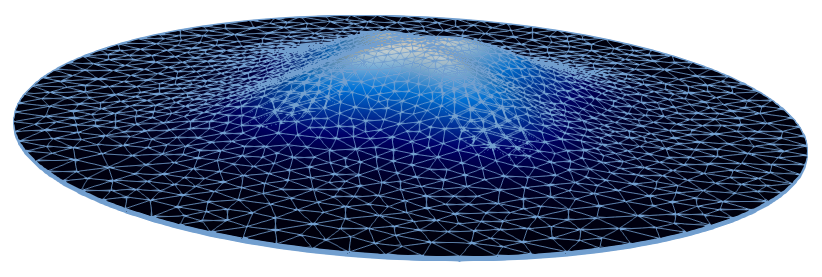
\includegraphics[scale=0.23]{meshHeight_view2_edges.png}
	\end{center}
	\caption{Ice sheet model geometry}
	\label{fig:ice_mountain_mesh}
    \end{subfigure} \\
	\begin{subfigure}{0.49\textwidth}
		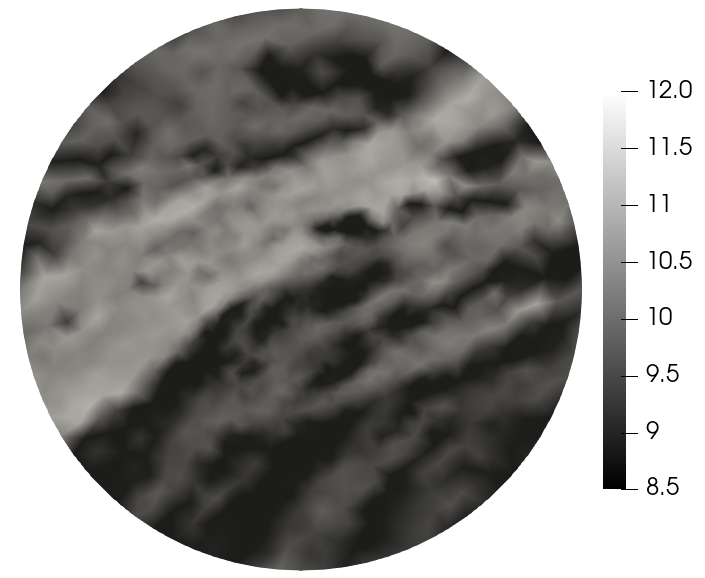
\includegraphics[scale=0.22]{mtrue_withColorBar.png}
		\caption{$\basalfriction_\text{true}$.}
		\label{fig:true_beta}
	\end{subfigure}
	\begin{subfigure}{0.49\textwidth}
		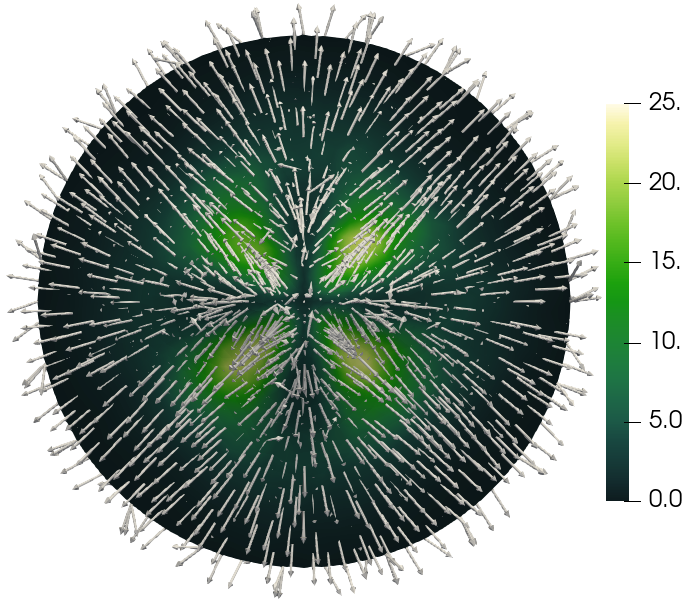
\includegraphics[scale=0.22]{trueVelocity2_glyphs.png}
		\caption{$\velocity_\text{true}$.}
		\label{fig:stokes_velocity}
	\end{subfigure}
    \end{center}
	\caption{(Ice sheet) 
		(\ref{fig:ice_mountain_mesh}) Bird's eye view of the ice sheet discretized by a mesh of tetrahedra. Color indicates the height of the base of the ice sheet (i.e., the mountain topography). The radius of the domain is $10^4$ meters, the maximum height of the mountain is $2.1 \times 10^3$ meters, and the average thickness of the ice sheet is 250 meters.		
		(\ref{fig:true_beta}) True parameter, $\basalfriction_\text{true}$. (\ref{fig:stokes_velocity}) True velocity, $\velocity_\text{true}$. Arrows indicate the direction of $\velocity_\text{true}$ and color indicates the magnitude of $\velocity_\text{true}$.}
	\label{fig:true_beta_u}
\end{figure} 


\begin{figure}
	\begin{subfigure}{0.32\textwidth}
		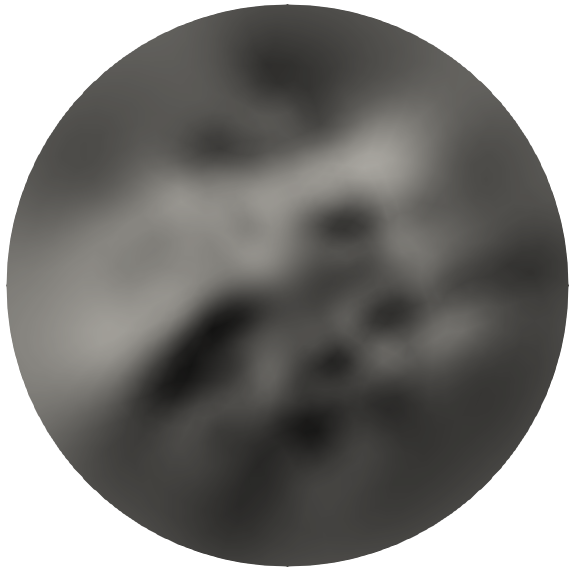
\includegraphics[scale=0.20]{mstar_0.25noise_cropped.png}
	\end{subfigure}
	\begin{subfigure}{0.32\textwidth}
		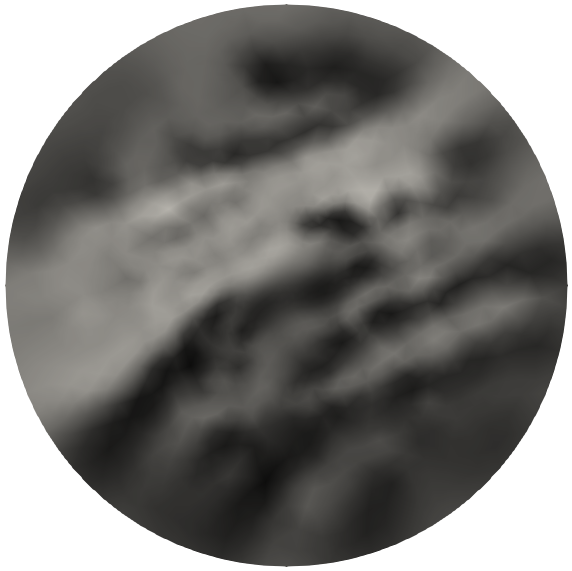
\includegraphics[scale=0.20]{mstar_0.05noise_cropped.png}
	\end{subfigure}
	\begin{subfigure}{0.32\textwidth}
	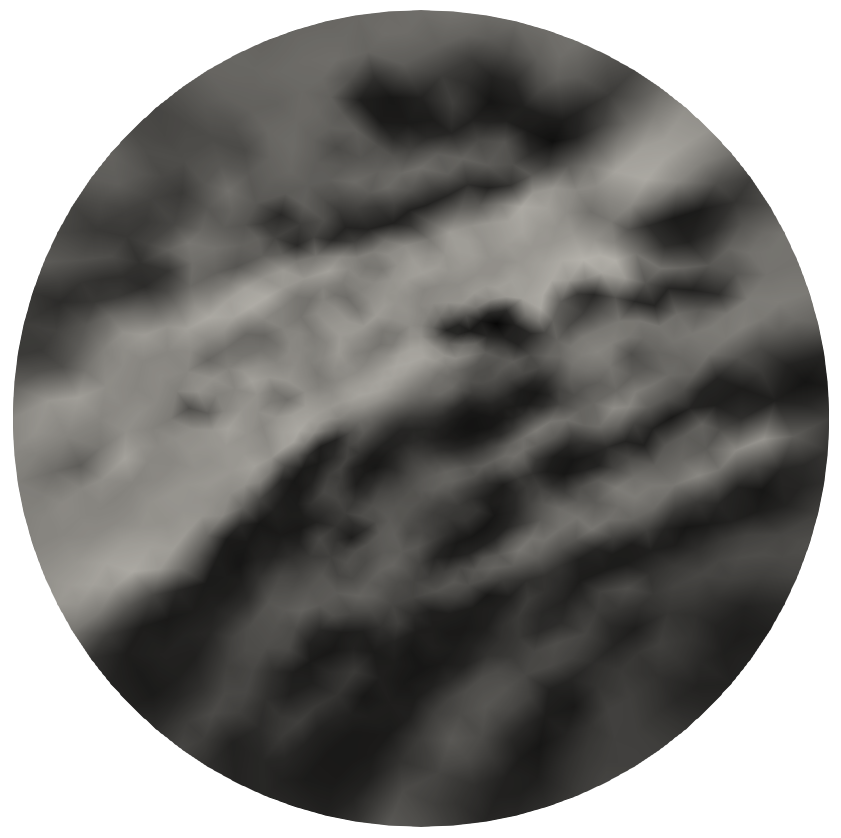
\includegraphics[scale=0.20]{mstar_0.01noise_cropped.png}
    \end{subfigure}
	\caption{(Ice sheet) The log basal friction parameter, with color scale as in Figure~\ref{fig:true_beta}, computed from the PDE-constrained optimization problem with noise levels: $25\%$ (left), $5.0\%$ (middle), and $1.0\%$ (right).}
	\label{fig:stokes_reconstructions} 
\end{figure} 

\begin{table}
	{\small
		\begin{center}
			\begingroup
			\setlength{\tabcolsep}{3pt}
			\renewcommand{\arraystretch}{1.1}
			\begin{tabular}{c| c c c | c c c | c c c}
				&  \multicolumn{3}{|c|}{PSF (5)} & \multicolumn{3}{|c|}{REG} & \multicolumn{3}{|c}{NONE} \\
				\hline
				Iter & 
				\#CG & \#Stokes & $\|\bm{g}\|$ & 
				\#CG & \#Stokes & $\|\bm{g}\|$ & 
				\#CG & \#Stokes & $\|\bm{g}\|$ \\
				0 &
				1 & 4 & 1.9e+7 &
				3 & 8 & 1.9e+7 &
				1 & 4 & 1.9e+7 \\
				1 &
				2 & 6  & 6.1e+6 &
				8 & 18 & 8.4e+6 &
				2 & 6  & 6.1e+6 \\
				2 &
				4 & 10 & 2.6e+6 &
				16 & 34 & 4.1e+6 &
				4 & 10 & 2.6e+6 \\
				3 &
				2 & 6+22 & 6.9e+5 &
				34 & 70 & 1.8e+6 &
				14 & 30 & 6.9e+5 \\
				4 &
				3 & 8 & 4.4e+4 &
				52 & 106 & 5.6e+5 &
				29 & 60 & 1.3e+5 \\
				5 &
				5 & 12 & 2.2e+3 &
				79 & 160 & 9.4e+4 &
				38 & 78 & 1.0e+4 \\
				6 &
				0 & 2 & 1.1e+1 &
				102 & 206 & 6.5e+3 &
				58 & 118 & 1.8e+2 \\
				7 &
				--- & --- & --- &
				151 & 304 & 1.2e+2 &
				0 & 2 & 5.5e-1 \\
				8 & 
				--- & --- & --- &
				0 & 2 & 2.9e-1 &
				--- & --- & --- \\
				\hline
				Total & 
				17 & 70 & --- &
				445 & 908 & --- &
				146 & 308 & --- \\
			\end{tabular}
			\endgroup
		\end{center}
	}
	\caption{(Ice sheet) Convergence history for solving the Stokes inverse problem using inexact Newton PCG. The Newton iteration is terminated when $||\mathbf{g}|| < 10^{-6} ||\mathbf{g}_0||$, where $\mathbf{g}$ is the gradient at the current iteration, and $\mathbf{g}_0$ is the gradient at the initial guess. Preconditioners shown are the proposed PSF method with five batches (PSF (5)) constructed at the third iteration, regularization preconditioning (REG), and no preconditioning (NONE). Columns titled \#CG show the number of PCG iterations used to solve the Newton system for $\bm{\widehat{\basalfriction}}$. Columns titled $\|\bm{g}\|$ show the $l^2$ norm of the gradient at $\bm{\basalfriction}$. Columns titled \#Stokes show the total number of Stokes PDE solves performed in each Newton iteration. This consists of Stokes solves performed during the line search to arrive at the current iterate from the previous iterate, plus one adjoint Stokes solve to compute the gradient at the current iterate, plus two Stokes solves per PCG iteration when solving the Newton system to compute the next search direction. Under PSF (5) and in row Iter 3, we write $6+22$ to indicate that $6$ Stokes solves were used during the standard course of the iteration, and $22$ Stokes solves were used to build the PSF (5) preconditioner.}
	\label{tab:newton_convergence_table}
\end{table}

Table~\ref{tab:newton_convergence_table} shows the performance of the preconditioner for accelerating the solution of the optimization problem to reconstruct $\mathbf{q}$ from observations with $5\%$ noise. We build the PSF (5) preconditioner in the third Gauss-Newton iteration, and reuse it for all subsequent Gauss-Newton and Newton iterations. No preconditioning is used in the Gauss-Newton iterations before the PSF (5) preconditioner is built. We compare the proposed method with the most commonly used existing preconditioners: no preconditioning (NONE), and preconditioning by the regularization term in the Hessian (REG). The results show that using PSF (5) reduces the total number of Stokes PDE solves substantially compared to regularization preconditioning and no preconditioning. In Figure~\ref{fig:stokes_reconstructions} we show reconstructions for $1\%$, $5\%$, and $25\%$ noise.
%
%
\begin{figure}
	\begin{subfigure}{0.52\textwidth}
		\centering
		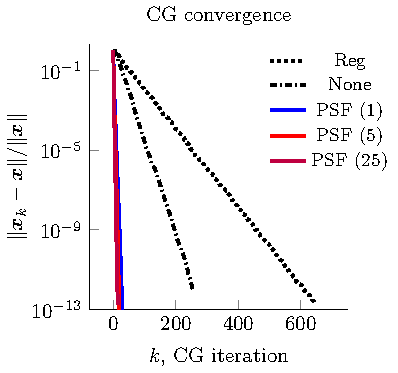
\includegraphics[scale=1.0]{stokes_pcg_convergence.pdf}
	\end{subfigure}
	\begin{subfigure}{0.47\textwidth}
	\begin{center}
		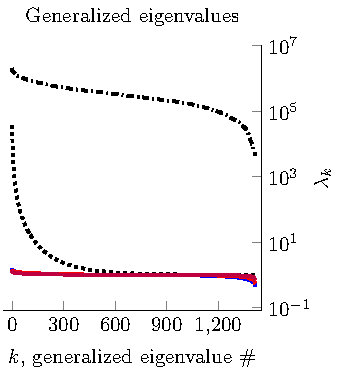
\includegraphics[scale=1.0]{stokes_geigs_figure.pdf}
	\end{center}
    \end{subfigure}
	\caption{(Ice sheet) Left: convergence history for solving $\bm{H} \bm{x} = \bm{b}$ using PCG, where $\bm{b}$ has i.i.d. random entries drawn from the standard Gaussian distribution and $\bm{H}$ is evaluated at the solution of the inverse problem. 
	Results in these figures are shown for the PSF-based preconditioners with 1, 5, and 25 batches (PSF (1), PSF (5), and PSF(25), respectively), regularization preconditioning (REG), and no preconditioning (NONE). The preconditioner is constructed using $\bm{H}_\text{gn}$.
	Right: generalized eigenvalues for generalized eigenvalue problem $\bm{H} \bm{u}_{k}=\lambda_{k} \bm{\preconditioner} \bm{u}_{k}$. Here $\bm{H}$ is the Hessian and $\bm{\preconditioner}$ is the PSF approximation constructed using the Gauss-Newton Hessian, $\bm{H}_\text{gn}$, for 1, 5, and 25 batches (PSF (1), PSF (5), and PSF (25), respectively), the regularization Hessian (REG), or the identity matrix (NONE).}
	\label{fig:krylov_convergence}
\end{figure} 
%

Next, we build PSF (1), PSF (5), and PSF (25) preconditioners based on the Gauss-Newton Hessian evaluated at the converged solution $\bm{\basalfriction}$. We use PCG to solve a linear system with the Hessian as the coefficient operator and a right hand vector with random independent and identically distributed (i.i.d.) entries drawn from the standard Gaussian distribution. In Figure~\ref{fig:krylov_convergence} (left) we compare the convergence of PCG for solving this linear system using the PSF (1), PSF (5), PSF (25), REG, and NONE preconditioners. PCG converges fastest with the PSF-based preconditioners, with PSF (25) converging fastest, followed by PSF (5), followed by PSF (1), as expected. 
In Figure~\ref{fig:krylov_convergence} (right) we show the generalized eigenvalues for the generalized eigenvalue problem
$
\bm{H} \mathbf{u} = \lambda \bm{\preconditioner} \mathbf{u}.
$ 
The matrix $\bm{\preconditioner}$ is one of the PSF (1), PSF (5), or PSF (25) Gauss-Newton Hessian approximations, the regularization Hessian (REG), or the identity matrix (NONE). With the PSF-based preconditioners, the generalized eigenvalues cluster near one, with more batches yielding better clustering. 

In Table~\ref{tab:condition_number}, we show the condition number of the preconditioned Hessian for a variety of noise levels ranging from $1\%$ to $25\%$. Note that the condition number using PSF-based preconditioners is extremely small (ranging between 1 and 10) and relatively stable over this range of noise levels. As expected, PSF (25) outperforms than PSF (5), which outperforms than PSF (1). All PSF-based preconditioners outperform no preconditioning and regularization preconditioning for all noise levels. 

\begin{table}
	\begin{center}
			\begingroup
			\setlength{\tabcolsep}{4pt}
			\renewcommand{\arraystretch}{1.25}
			\begin{tabular}{c| c c c c c}
				noise    & \multicolumn{5}{c}{COND$(\bm{\preconditioner}^{-1} \bm{H})$ } \\ \cline{2-6}
				level    & REG     &	NONE  & PSF $(1)$ & PSF $(5)$ & PSF $(25)$ \\ \hline 
				$25\%$   & 1.01e+3 & 2.96e+3  & 1.34e+0   & 1.30e+0   & 1.18e+0    \\ 
				$11\%$   & 7.40e+3 & 1.05e+3  & 2.27e+0   & 1.55e+0   & 1.31e+0    \\   
				$5.0\%$  & 3.29e+4 & 4.96e+2  & 5.61e+0   & 3.06e+0   & 1.92e+0    \\ 
				$2.2\%$  & 1.66e+5 & 8.89e+2  & 1.58e+1   & 8.07e+0   & 4.03e+0    \\  
				$1.0\%$  & 5.36e+5 & 1.61e+3  & 7.17e+1   & 1.93e+1   & 9.19e+0    \\   
			\end{tabular}
			\endgroup
		\end{center}
	\caption{(Ice sheet) Condition number for $\bm{\preconditioner}^{-1} \bm{H}$ for the PSF-based preconditioners with 1, 5, and 25 batches (PSF (1), PSF (5), and PSF(25), respectively), no preconditioner (NONE) and regularization (REG). All operators are evaluated at the soutions of the inverse problems for 
	their respective noise levels.}
	\label{tab:condition_number}
\end{table}



\subsection{Example 2: Inversion for the initial condition in an diffusive transport problem}
\label{sec:adv}

Here we consider a time-dependent advection-diffusion equation in
which we seek to infer the unknown spatially varying initial condition, $\ipar$, from noisy observations of the state  
at a final time, $T$. This PDE
models diffusive transport in a domain $\advdomain \subset \R^d$, which is
depicted in Figure~\ref{fig:adv_inversion1}. In this case, the state, $\concentration(x,t)$, could be interpreted as the concentration of a contaminant. The problem description
below closely follows the one in~\cite{PetraStadler11}. The domain
boundaries $\partial \advdomain$ include the outer boundaries as well as the
internal boundaries of the rectangles, which represent buildings.  The
parameter-to-observable map $\iFF$ in this case maps an initial
condition $\ipar \in L^2(\advdomain)$ to observations of the concentration at a final time, $\concentration(x, T)$,  through solution of the advection-diffusion
equation given by
\begin{equation}\label{eq:ad}
  \begin{aligned}
    \concentration_t - \kappa\Delta \concentration + v\cdot\nabla \concentration &= 0 & \quad&\text{in
    }\advdomain\times (0,T), \\
    \concentration(\cdot, 0) &= \ipar  &&\text{in } \advdomain , \\
    \kappa\nabla \concentration\cdot \nu &= 0 &&\text{on } \partial \advdomain \times (0,T).
  \end{aligned}
\end{equation}
Here, $\kappa > 0$ is a diffusivity coefficient, $\nu$ is the boundary unit normal vector, and $T > 0$ is the
final time.  The velocity field, $v:\advdomain \rightarrow \mathbb{R}^d$, is computed by solving the
steady-state Navier-Stokes equations for a two dimensional flow with
Reynolds number 50, with boundary conditions $v(x)=(0,1)$ on the left boundary, $v(x)=(0,-1)$ on the right boundary, and $v(x)=(0,0)$ on the top and bottom boundaries, as in~\cite[Section 3]{PetraStadler11}. We use a checkerboard image for the initial condition (Figure~\ref{fig:adv_initial_condition}) and add $5\%$ multiplicative noise to generate synthetic observations at the final time, $T$. The initial condition, velocity field, noisy observations, and reconstructed initial condition are shown in Figure~\ref{fig:adv_inversion1}. We use $\kappa=3.2$e${-1}$ and $T=1.0$ for all results, except for Table \ref{tab:adv_convergence} and Figure~\ref{tbl:adv_vary_kappa_tf} where we vary $\kappa$ and $T$.

In Table~\ref{tab:adv_convergence} we show the number of PCG iterations, $j$, required to solve the Newton linear system to a relative error tolerance of $\|\widehat{\mathbf{q}} - \widehat{\mathbf{q}}_j\| < 10^{-6} \|\widehat{\mathbf{q}}\|$. The solution of the Newton system that we compare to, $\widehat{\mathbf{q}}$, is found via another PCG iteration with a relative residual tolerance of $10^{-11}$. We show results for $T$ ranging from $0.5$ to $2.0$ and $\kappa$ ranging from $10^{-4}$ to $10^{-3}$ using the PSF-based preconditioners with $1$, $5$, and $25$ batches, regularization preconditioning, and no preconditioning. The results show that PSF-based preconditioning outperforms regularization preconditioning and no preconditioning, with more batches yielding better results. 


In Figure~\ref{fig:adv_krylov_convergence} (left) we show the convergence of PCG for solving $\bm{H}\bm{x}=\bm{b}$, where $\bm{b}$ has i.i.d. random entries drawn from a standard Gaussian distribution. The preconditioners used, $\widetilde{\bm{H}}$, are the PSF-based preconditioners with $1$, $5$, or $25$ batches, the regularization Hessian, and the identity matrix (i.e., no preconditioning). The results show that PCG converges fastest with the PSF-based preconditioners, with more batches yielding faster convergence. In Figure~\ref{fig:adv_krylov_convergence} (right), we show the eigenvalues for the generalized eigenvalue problem $\bm{H}\bm{u}=\lambda \widetilde{\bm{H}}\bm{u}$, where the $\widetilde{\bm{H}}$ are the preconditioners stated above. With the PSF-based preconditioners the eigenvalues cluster near one, and more batches yields better clustering. With the regularization preconditioner the trailing eigenvalues cluster near one, while the leading eigenvalues are amplified.

\begin{figure}
	\begin{center}
	\begin{subfigure}{0.24\textwidth}
		\begin{center}
		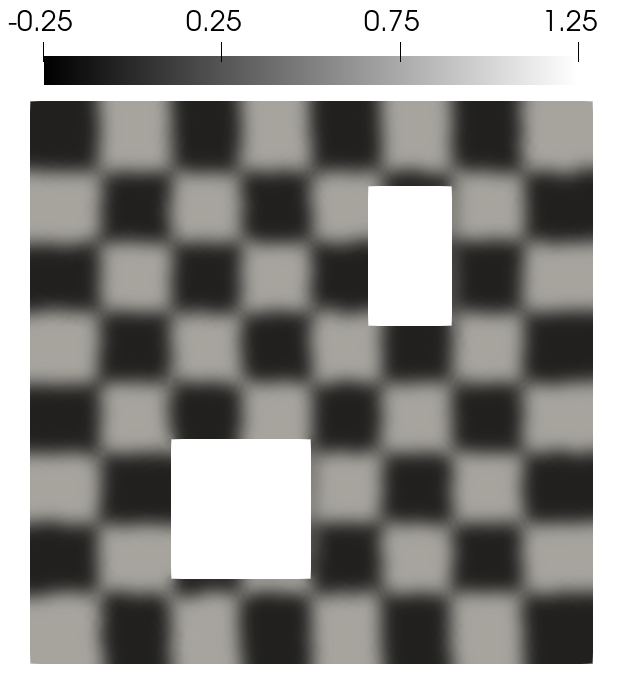
\includegraphics[scale=0.14]{true_initial_condition.png}
	\end{center}
				\caption{True $q$}
				\label{fig:adv_initial_condition}
	\end{subfigure}
	\begin{subfigure}{0.24\textwidth}
		\begin{center}
		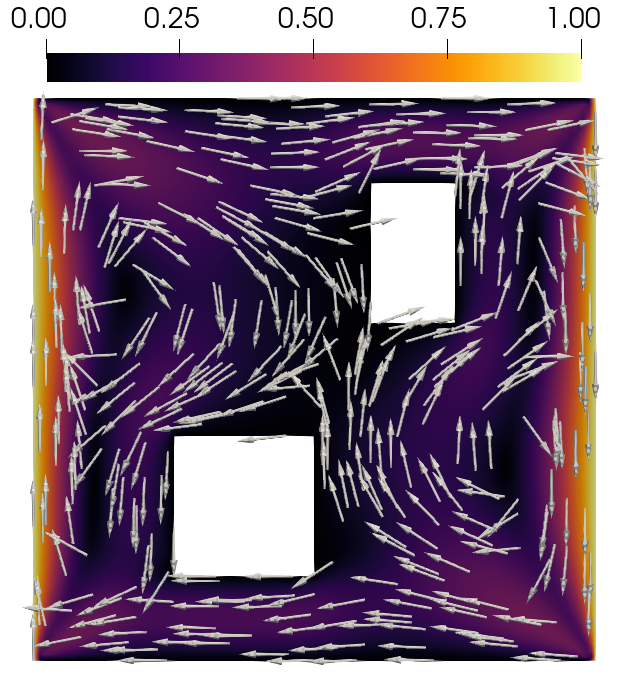
\includegraphics[scale=0.14]{wind_velocity_colorscheme3.png}
		\end{center}
				\caption{$v$}
				\label{fig:adv_velocity}
	\end{subfigure}
	\begin{subfigure}{0.24\textwidth}
		\begin{center}
		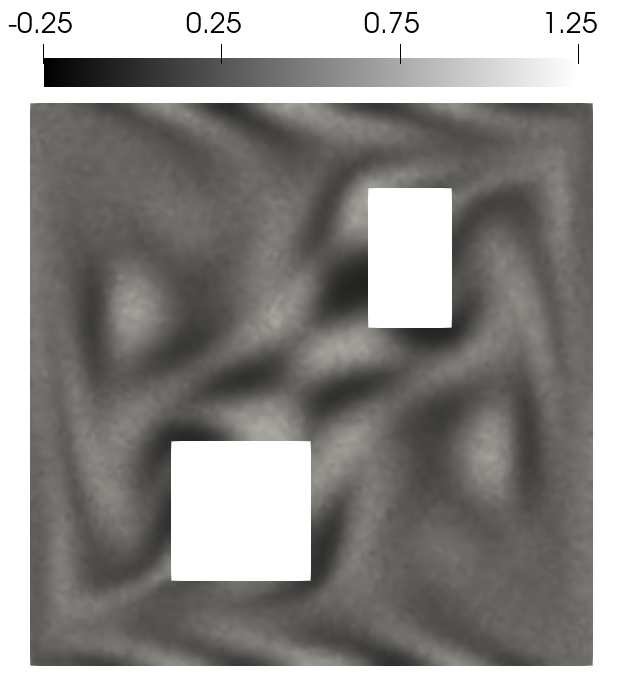
\includegraphics[scale=0.14]{noisy_observations_T1.0_K3.2e-4.png}
		\end{center}
				\caption{Noisy observations}
				\label{fig:adv_observations}
	\end{subfigure}
	\begin{subfigure}{0.24\textwidth}
		\begin{center}
		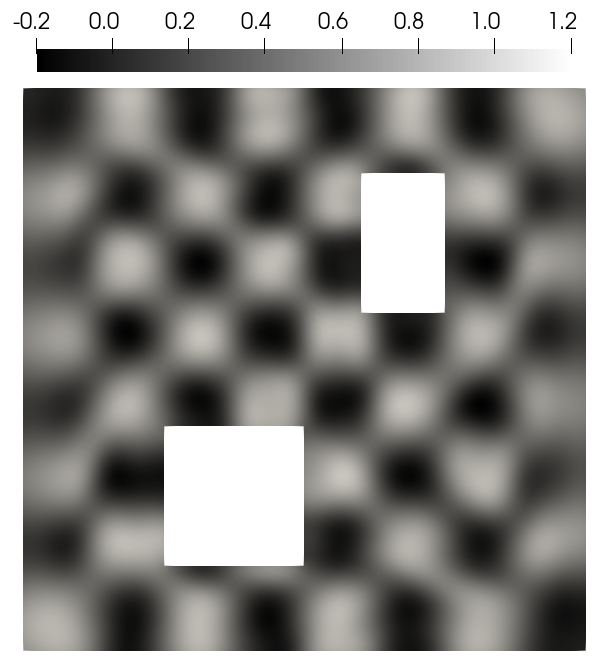
\includegraphics[scale=0.14]{reconstructed_initial_condition_T1.0_K3.2e-4.png}
		\end{center}
				\caption{Reconstructed $q$}
				\label{fig:adv_reconstruction}
	\end{subfigure}
	\end{center}
	\caption{(Diffusive transport) (\ref{fig:adv_initial_condition}) True initial condition. (\ref{fig:adv_velocity}) Velocity field. Color indicates magnitude of velocity vector. (\ref{fig:adv_observations}) Noisy observations of concentration at final time. (\ref{fig:adv_reconstruction}) Reconstructed initial condition.}
	\label{fig:adv_inversion1} 
\end{figure} 

\begin{table}
	\begin{center}
		\begingroup
		\setlength{\tabcolsep}{8pt}
		\renewcommand{\arraystretch}{1.0}
		\begin{tabular}{c| c | c c c c c}
			& $\kappa$    & REG     &	NONE   & PSF $(1)$ & PSF $(5)$ & PSF $(25)$ \\ 
			\hline 
			& 1.0e-4    & 584 & 317  & 311   & 151   & 56    \\ 
			%			& $1.8e{-4}$    & 628 & 313  & 192   & 131   & 49    \\   
			$T=0.5$ & 3.2e-4    & 685 & 311  & 233   & 140   & 44    \\ 
			%			& $5.6e{-4}$    & 734 & 310  & 334   & 144   & 40    \\  
			& 1.0e-3    & 702 & 324  & 122   & 71   & 33    \\ 
			\hline
			& 1.0e-4    & 634 & 449  & 539   & 288   & 100    \\ 
			%			& $1.8e{-4}$    & 665 & 449  & 493   & 212   & 84    \\   
			$T=1.0$ & 3.2e-4    & 681 & 459  & 350   & 202   & 90    \\ 
			%			& $5.6e{-4}$    & 619 & 482  & 262   & 197   & 70    \\  
			& 1.0e-3    & 574 & 520  & 266   & 260   & 208    \\ 
			\hline
			& 1.0e-4    & 609 & 591  & 548   & 520   & 165    \\ 
			%			& 1.8e{-4}$    & 576 & 611  & 434   & 426   & 185    \\   
			$T=2.0$ & 3.2e-4    & 524 & 645  & 318   & 379   & 170    \\ 
			%			& $5.6e{-4}$    & 464 & 711  & 480   & 289   & 153    \\  
			& 1.0e-3    & 349 & 786  & 381   & 262   & 158    \\ 
		\end{tabular}
		\endgroup
	\end{center}
	\caption{(Diffusive transport) Number of PCG iterations required to solve the Newton linear system to tolerance $||\widehat{\bm{q}}_j - \widehat{\bm{q}}|| < 10^{-6}||\widehat{\bm{q}}||$, where $\widehat{\bm{q}}_j$ is the $j$th iterate, and $\widehat{\bm{q}}$ is the solution of the Newton linear system. Iteration counts are shown for a variety of different diffusion parameters $\kappa$, simulation times $T$, and preconditioners.}
	\label{tab:adv_convergence}
\end{table}


\begin{figure}
	\centering
	{
		%	\setlength{\tabcolsep}{0.1em}
		%	\renewcommand{\arraystretch}{2.0}
		\begin{tabular}{ccc}
			& $T=0.5$ 
%			& $T=1.0$ 
			& $T=2.0$ \\
			$\kappa=1.0$e${-4}$  & 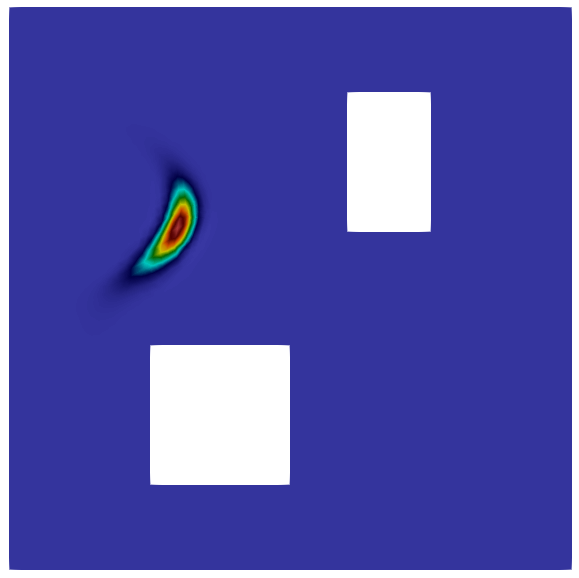
\includegraphics[scale=0.15, valign=c]{impulse_response_P(0.3,0.6)_T0.5_K1.e-4.png} 
%			& 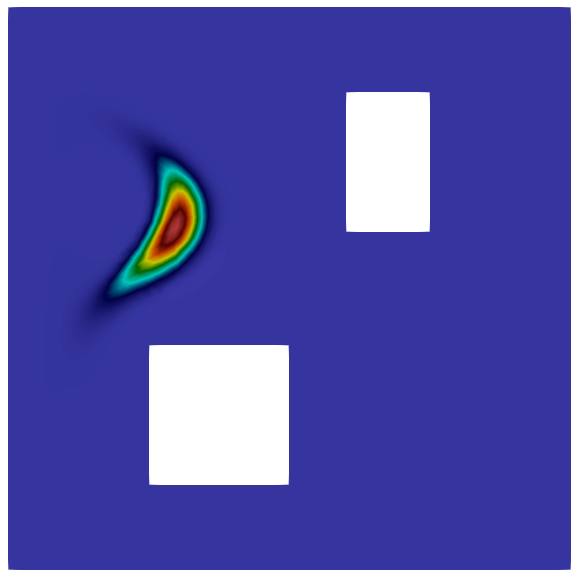
\includegraphics[scale=0.15, valign=c]{impulse_response_P(0.3,0.6)_T1.0_K1.e-4.png}
			& 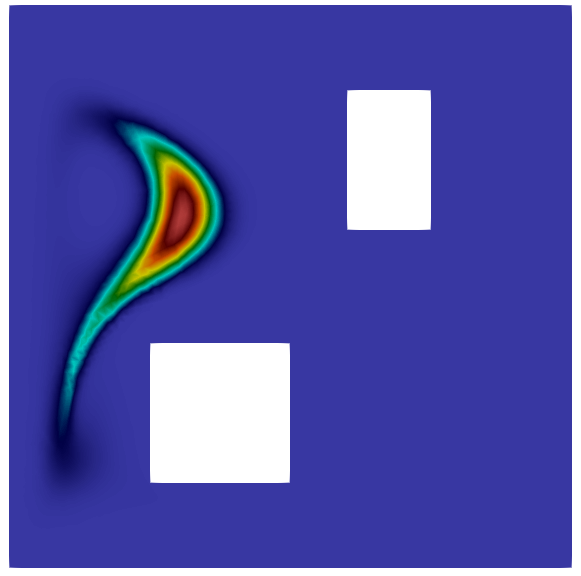
\includegraphics[scale=0.15, valign=c]{impulse_response_P(0.3,0.6)_T2.0_K1.e-4.png} \\
%			$\kappa=3.2$e${-4}$ & 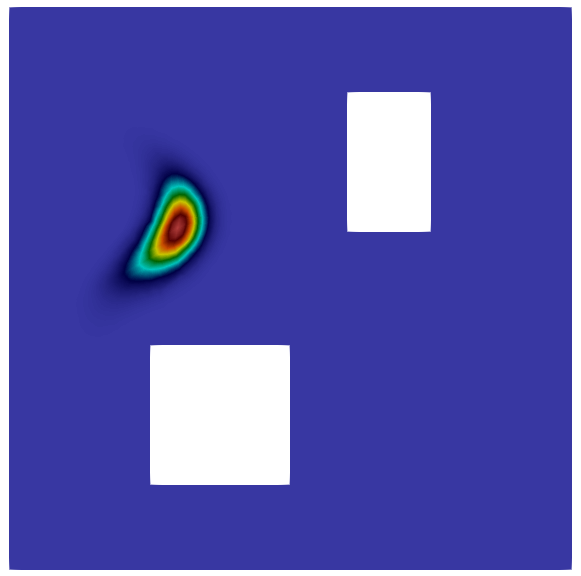
\includegraphics[scale=0.15, valign=c]{impulse_response_P(0.3,0.6)_T0.5_K3.2e-4.png} & 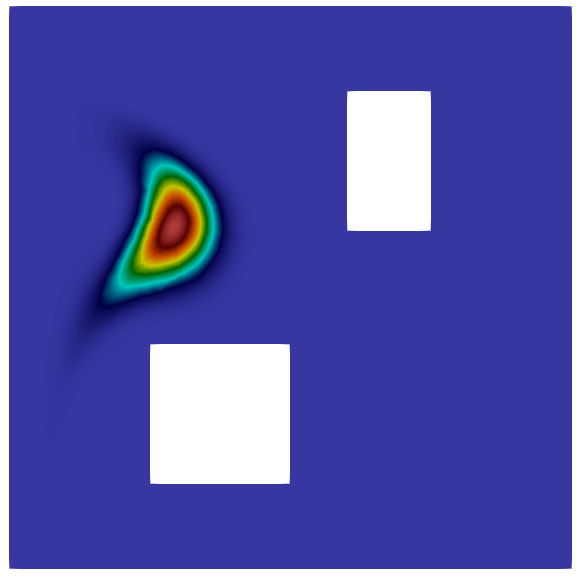
\includegraphics[scale=0.15, valign=c]{impulse_response_P(0.3,0.6)_T1.0_K3.2e-4.png} & 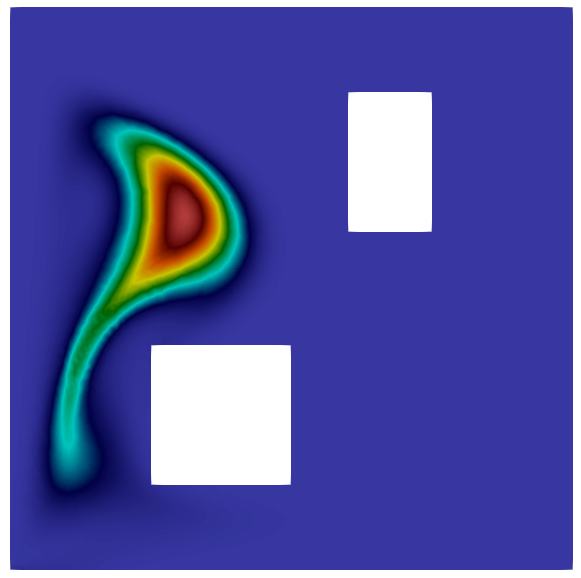
\includegraphics[scale=0.15, valign=c]{impulse_response_P(0.3,0.6)_T2.0_K3.2e-4.png} \\
			$\kappa=1.0$e${-3}$ & 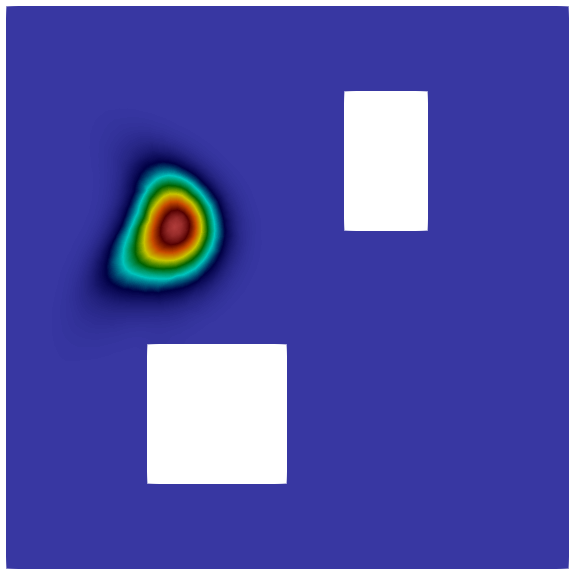
\includegraphics[scale=0.15, valign=c]{impulse_response_P(0.3,0.6)_T0.5_K1.e-3.png} 
%			& 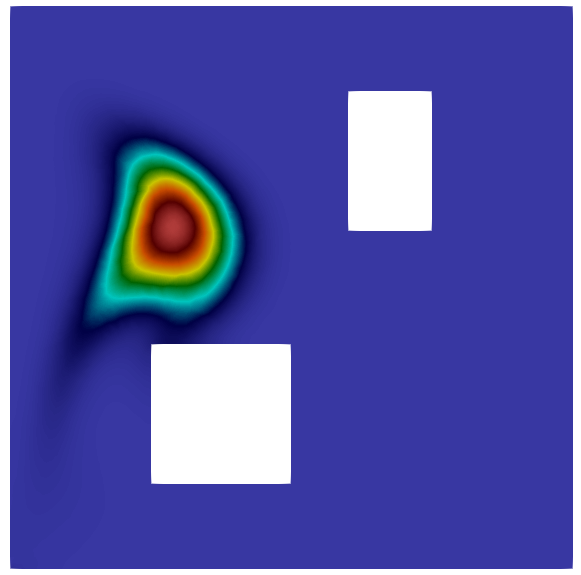
\includegraphics[scale=0.15, valign=c]{impulse_response_P(0.3,0.6)_T1.0_K1.e-3.png} 
			& 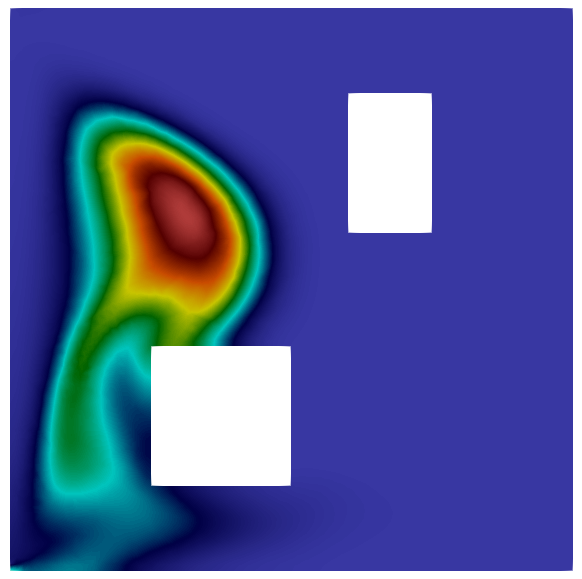
\includegraphics[scale=0.15, valign=c]{impulse_response_P(0.3,0.6)_T2.0_K1.e-3.png}
		\end{tabular}
	}
	\caption{(Diffusive transport) Impulse responses for small and large diffusion parameters $\kappa$ and simulation times $T$.}
	\label{tbl:adv_vary_kappa_tf}
\end{figure}


\begin{figure}
	\begin{subfigure}{0.52\textwidth}
		\centering
		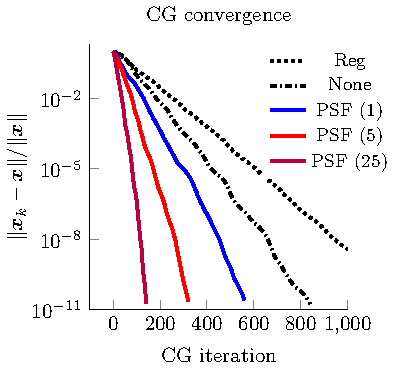
\includegraphics[scale=1.0]{adv_pcg_convergence.pdf}
	\end{subfigure}
	\begin{subfigure}{0.47\textwidth}
		\centering
		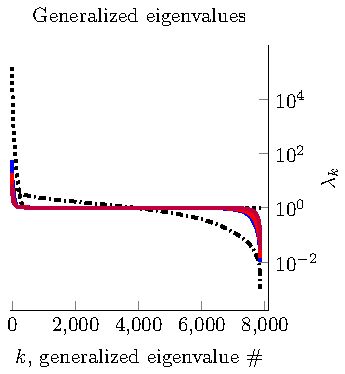
\includegraphics[scale=1.0]{adv_geigs_figure.pdf}
	\end{subfigure}
	\caption{(Diffusive transport) Left: convergence history for solving $\bm{H} \bm{x} = \bm{b}$ using PCG, where $\bm{b}$ has i.i.d. random entries drawn from the standard Gaussian distribution. Right: generalized eigenvalues for generalized eigenvalue problem $\bm{H} \bm{u}_{k}=\lambda_{k} \bm{\preconditioner} \bm{u}_{k}$. Here $\bm{H}$ is the Hessian and the preconditioner $\bm{\preconditioner}$ is the PSF approximation for 1, 5, or 25 batches (PSF (1), PSF (5), and PSF (25), respectively), the regularization Hessian (REG), or the identity matrix (NONE).}
	\label{fig:adv_krylov_convergence}
\end{figure} 


\section{Conclusions}
\label{sec:conclusions}

We presented an efficient matrix-free PSF method for approximating operators with locally supported non-negative integral kernels. The method only requires access to the operator via application of the operator to a small number of vectors. The idea of the method is to compute batches of impulse responses by applying the operator to Dirac combs of scattered point sources, then interpolate these impulse responses to approximate entries of the operator's integral kernel. The interpolation is based on a new principle we call ``local mean displacement invariance,'' which generalizes classical local translation invariance. The ability to quickly approximate arbitrary integral kernel entries permits us to form an H-matrix approximation of the operator. Fast H-matrix arithmetic is then used to perform further linear algebra operations that cannot be performed easily with the original operator, such as matrix factorization and inversion. The supports of the impulse responses are estimated to be contained in ellipsoids, which are determined a-priori via a moment method that involves applying the operator to a small number of polynomial functions. Point source locations for the impulse response batches are chosen using a greedy ellipsoid packing procedure, in which we choose as many impulse responses per batch as possible, while ensuring that the corresponding ellipsoids do not overlap. We applied the method to approximate the Gauss-Newton Hessians in an ice sheet flow inverse problem governed by the Stokes PDE, and a diffusive transport inverse problem governed by an advection-diffusion PDE. We saw that the proposed approximation method substantially outperforms existing Hessian approximation methods. Although the method we presented is not applicable to all Hessians, it is applicable to many Hessians of practical interest. For these Hessians, the proposed method offers a \emph{data scalable} alternative to conventional low rank approximation, due to the ability to form high rank approximations of an operator using a small number of operator applications, and thus forward and adjoint PDE solves.


\section*{Acknowledgments}
We thank J.J. Alger, Longfei Gao, Mathew Hu, and Rami Nammour for helpful discussions. We thank Trevor Heise for editing suggestions. We thank Georg Stadler for help with the domain setup for the ice sheet problem.

\FloatBarrier

\bibliographystyle{siamplain}
\bibliography{localpsf}

\end{document}
